% This document provides the style to be used for a MSc Thesis at the
% Parallel and Distributed Systems group
\documentclass[11pt,twoside,a4paper,openright]{report}

% use babel for proper hyphenation
\usepackage[british]{babel}
% Graphics: like the DUT logo on the front cover
\usepackage[dvips]{graphicx}
%Enables [H] for figures.
\usepackage{float}
% FONT: times
\usepackage{times}
% for url's use "\url{http://www.google.com/}"
\usepackage{url}
% To allow margin adjustments
\usepackage{changepage}
% To allow listings.
\usepackage{listings}
% To inserts to do's
\usepackage{todonotes}
% Boxed verbatim for experiments
\usepackage{fancyvrb}
% Side by side packages
%\usepackage{subfigure}
% sub caption package
\usepackage{subcaption}
% csquote for quotes
\usepackage{csquotes}
% Multirow for multirow tables
\usepackage{multirow}
% bib in order of appearance
\bibliographystyle{ieeetr}
% Symbols for checkmarks and cross marks.
\usepackage{amssymb}% http://ctan.org/pkg/amssymb
\usepackage{pifont}% http://ctan.org/pkg/pifont
\newcommand{\cmark}{\ding{51}}
\newcommand{\xmark}{\ding{55}}

\newsavebox{\FVerbBox}
\newenvironment{FVerbatim}
 {\VerbatimEnvironment
  \begin{center}
  \begin{lrbox}{\FVerbBox}
  \begin{BVerbatim}}
 {\end{BVerbatim}
  \end{lrbox}
  \fbox{\usebox{\FVerbBox}}
  \end{center}}
  
  
%%%%%%%%%%%%%%%%%%%%%%%%%%%%%%%%%%%%%%%%%%%%%%%%%%%%%%%%%%%%%
 % Listing markup
 \lstset{ %
 	language=xml,
 	basicstyle=\footnotesize,       % the size of the fonts that are used for the code
 	numbers=none,                   % where to put the line-numbers
 	xleftmargin=2em,
 	numberstyle=\footnotesize,      % the size of the fonts that are used for the line-numbers
 	stepnumber=2,                   % the step between two line-numbers. If it's 1, each line will be numbered
 	numbersep=5pt,                  % how far the line-numbers are from the code
 	backgroundcolor=\color{white},  % choose the background color. You must add \usepackage{color}
 	showspaces=false,               % show spaces adding particular underscores
 	showstringspaces=false,         % underline spaces within strings
 	showtabs=false,                 % show tabs within strings adding particular underscores
 	frame=single,                   % adds a frame around the code
 	tabsize=2,                      % sets default tabsize to 2 spaces
 	captionpos=b,                   % sets the caption-position to bottom
 	breaklines=true,                % sets automatic line breaking
 	breakatwhitespace=false,        % sets if automatic breaks should only happen at whitespace
 	title=\lstname,                 % show the filename of files included with \lstinputlisting;
 	% also try caption instead of title
 	escapeinside={(*}{*)},         % if you want to add a comment within your code
 	morekeywords={*,...},            % if you want to add more keywords to the set
 	keywordstyle=\color[rgb]{0,0,1},
 	commentstyle=\color[rgb]{0.133,0.545,0.133},
 	stringstyle=\color[rgb]{0.627,0.126,0.941}
 }
 
%%%%%%%%%%%%%%%%%%%%%%%%%%%%%%%%%%%%%%%%%%%%%%%%%%%%%%%%%%%%%

\begin{document}

%%%%%%%%%%%%%%%%%%%%%%%%%%%%%%%%%%%%%%%%%%%%%%%%%%%%%%%%%%%%%%%%%%%%%%%%%%%%%%%
\hoffset=1.63cm
\oddsidemargin=0in
\evensidemargin=0in
\textwidth=5in

%%%%%%%%%%%%%%%%%%%%%%%%%%%%%%%%%%%%%%%%%%%%%%%%%%%%%%%%%%%%%%%%%%%%%%%%%%%%%%%
% No identing
\setlength\parindent{0pt}

\pagestyle{empty}

% FRONTCOVER
\begin{titlepage}

\null\vfill

\begin{center}
\LARGE{Software Performance Engineering in Complex Distributed Systems}
\end{center}

\vspace{1.5cm}

\begin{center}
Laurens F. D. Versluis\\
L.F.D.Versluis@student.tudelft.nl
\end{center}

\vfill

\centering
\begin{figure}[!b]
\captionsetup[subfigure]{labelformat=empty}
\begin{subfigure}{0.4\textwidth}
\centering

\includegraphics[height=3cm]{pics/triblerlogo}
\caption{}
\end{subfigure}%
\begin{subfigure}{0.6\textwidth}
\centering
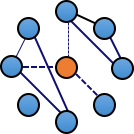
\includegraphics[height=3cm]{pics/dslogo}
\caption{}
\end{subfigure}%
\end{figure}

\begin{figure}[!b]
\centering

\includegraphics[height=2cm]{pics/TUDLogo}
\end{figure}


\vspace{2.0cm}

\end{titlepage}


% EMPTY PAGE
% \cleardoublepage

\pagestyle{plain}

% TITLE PAGE: page i (hidden)
\begin{titlepage}

  \begin{center}
  \null\vfill
    \begin{center}
    \LARGE{Software Performance Engineering in Complex Distributed Systems}
    \end{center}

    \vspace{3cm}

    \begin{large}
    Master's Thesis in Computer Science
    \end{large}

    \vspace{1.5cm}

    \begin{normalsize}
	Distributed Systems group\\
    Faculty of Electrical Engineering, Mathematics, and Computer Science\\
    Delft University of Technology
    \end{normalsize}

    \vspace{2.0cm}

    \begin{normalsize}
    Laurens F. D. Versluis
    \end{normalsize}

    \vspace{1.0cm}

    % <MM> DD, YYYY
    \today

  \vfill
  \end{center}

\end{titlepage}



% GRADUATION DATA AND ABSTRACT: pages ii and iii (hidden)
%De aankondiging bevat de spreker, titel, plaats, datum en tijd, samenstelling van de afstudeercommissie en een korte samenvatting (maximaal 25 regels).
\thispagestyle{empty}

\noindent \textbf{Author}\\
\begin{tabular}{l}
Laurens F. D. Versluis\\
\\
\end{tabular}\\
\noindent \textbf{Title}\\
\begin{tabular}{l}
Addressing database constrained self organizing \& distributed systems\\
\\
\end{tabular}\\
\noindent \textbf{MSc presentation}\\
\begin{tabular}{l}
% <MM> DD, YYYY (like \today)
Dijkstrazaal, HB09.150\\
EEMCS, Delft\\
15:00-16:00, August 29, 2016
\\
\end{tabular}

\vspace{1.1cm}

\noindent \textbf{Graduation Committee}\\
\begin{tabular}{ll}
% The order of listing the names: Graduation prof, supervisor(s), others ordered by title + alphabetical
%examples:
%prof. dr. ir. H. J. Sips (chair) & Delft University of Technology \\
%ir. dr. D. H. J. Epema           & Delft University of Technology \\
dr. ir. J. A. Pouwelse            & Delft University of Technology \\
dr. ir. M. Zuniga                 & Delft University of Technology \\
dr. ir. A. Bozzon                 & Delft University of Technology \\

\end{tabular}

\begin{abstract} %de abstract bevat alleen een korte samenvatting van de inhoud van het onderzoek
TBD.



\end{abstract}

% \clearpage



\pagenumbering{roman}
\setcounter{page}{4}

% EMPTY PAGE: page iv
% \cleardoublepage

% OPTIONAL QUOTATION: page v
%\pagestyle{empty}

\null\vfill

\begin{center}
\emph{``TODO QUOTE''} -- TODO QUOTED PERSON
\end{center}

\vspace{10cm}

\clearpage


% EMPTY PAGE: page vi
%\cleardoublepage

% PREFACE: page v
\chapter*{Preface}
\addcontentsline{toc}{chapter}{Preface}
This thesis presents the work I have conducted in the last ten months.
During this period, I have had the pleasure of meeting new people who made my time much more enjoyable.
I would like to thank some people who contributed to this thesis.
Firstly, I would like to thank Johan Pouwelse for offering me this thesis and providing feedback on my work.
Secondly, I would like to thank Elric Milon who shared his knowledge of Tribler, Python, Git and Emacs with me as well as maintaining and updating our infrastructure from which everyone profited.
Thirdly, I am grateful to Pim Otte for reviewing my work and providing feedback.
I would also like to thank both Martijn and Hans, who I have spent the most time with in the MSc lab and for occasionally helping me when struggling with Linux.
Next, I would like to thank Ernst, Niels, Paul and everyone else of the Tribler team for providing feedback and suggestions.
Last but not least, I would like to thank my friends and family for their support, motivation and encouragement throughout my thesis.

\vspace{1\baselineskip}

\noindent
Laurens Freydis Dene Versluis

\vspace{1\baselineskip}

\noindent
Delft, The Netherlands

\noindent
\today
% EMPTY PAGE: page vi
% \clearpage

% TABLE OF CONTENTS: starting at page vii
\setcounter{tocdepth}{2}
\tableofcontents

% \cleardoublepage

\pagenumbering{arabic}
\setcounter{page}{1}

% CHAPTERS ... For instance: History/Prior Work, Design/Implementation, Experiments
% INTRODUCTION
\chapter{Introduction}
\label{chp:introduction}
Tribler is a peer-to-peer BitTorrent client that attempts to fully decentralize downloading, uploading and streaming of content.

Tribler focusses on the goals:
\begin{itemize}
    \item Allow for secure and private communication and sharing of data.
    \item Enforce user contribution in the network
    \item Make it impossible to shut Tribler down, unless the Internet itself as a whole gets taken down.
\end{itemize}

A fully decentralized ecosystem i.e. no central components present, is Tribler's approach to achieve these goals.
Tribler has been designed and build with this focus~\cite{Pouwelse-tribler,Bakker-tribler}.
A distributed network requires both the presence and collaboration of participants, called peers, to be able to achieve this.

This thesis was conducted to improve the connectability and overall performance of Tribler, by identifying and removing bottlenecks present in the system.

\begin{figure}
	\centerline{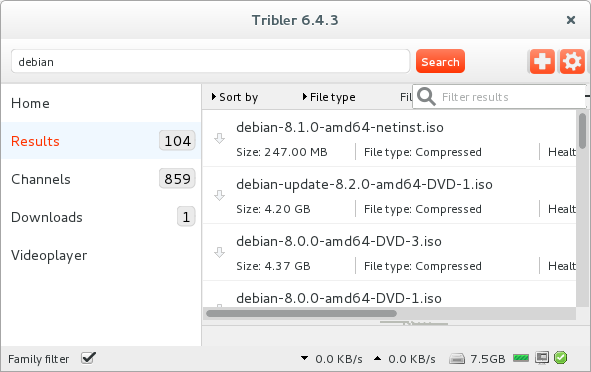
\includegraphics[scale=0.6]{introduction/figs/tribler-screenshot.png}}
	\caption{Screenshot of Tribler v6.4.3.}
	\label{fig:tribler-screenshot}
\end{figure}

\section{BitTorrent protocol}
When sharing files by using the BitTorrent protocol, a peer that uploads parts of a file to another peer, is called a seeder.
A peer that is downloading a file of a seeder is called a leecher.
Any peer can be both a seeder and leecher at the same time, and join the network at any given time.

The ratio between the total data downloaded and uploaded is called the seeding ratio \cite{Cohen-bittorrent}.
The seeding ratio can be seen as an indication of the level of collaboration i.e. giving back resources to the network.

Seeding can be seen as an interaction between peers, where the seeder aids the leeching peer.
By utilizing the seeders upload bandwith, the leeching peer can use his download bandwidth to download a file.
While there is a clear incentive for the leecher by downloading the desired file, there is none for the seeder.
Especially since the leecher has a little chance of becoming also be a seeder for the original seeder \cite{Lai-Incentives}.

Having peers actively and persistently contribute to the network will increase the network's health which in turn provides several benefits for all peers.
A more healthy network results in a higher availability of seeders and results in high download speeds.
It has been shown that private communities where the seeding ratio is high, provides better download conditions \cite{meulpolder-privatecommunities}.
In these private communities, trackers i.e. central components introduce peers to each other using the Tit-for-tat approach \cite{cohen-titfortat}.
The Tit-for-Tat approach is aiding peers who have aided you in the past,
The absence of trackers, which is often the case in public networks, results in free-riding \cite{Adar-Freeriding}.
A free-riding peer does not or gives little back to the network while receiving all benefits i.e. download without any restriction.
BitTorrent applies a variation of the Tit-for-tat strategy, optimistic chocking, to combat this problem.
The Tit-for-Tat strategy is to only provide help to peers that return this help.
% TODO explain the optimistic chocking approach
However, it has been shown that this approach is not effective in battling abuse \cite{Pouwelse-tribler}.

\section{Tribler}
Tribler wants to achieve a high global seeding ratio by making it beneficial to have such a ratio.
Nodes can award each other with higher cooperation if a node has a reputation of being cooperative,
while malicious nodes are prevented from tampering and freeriding.
Within Tribler anonymous connections have been implemented recently using onion routing~\cite{Plak-anonymous,ruigrok-anonymous,tanaskoski-anonymous}.
This feature allows downloaders to become indistinguishable from other users in the network save guarding their privacy.
Every data packet has to be forwarded
by a number of intermediate hops between the downloader and seeder~\cite{Plak-anonymous,tanaskoski-anonymous}.
The total cost of bandwidth per file is increased,
because it has to be forwarded by multiple nodes.
but also the number of nodes helping a single node downloading a file increases.
The increase in nodes working together increases the necessity of an incentive system to reward collaboration.

Dispersy is middleware for data dissemination in a network.
Dispersy is used heavily within Tribler and is maintained by the Tribler organisation.
Our work is build upon Dispersy.
Dispersy is used to exchange data between two specific nodes~\cite{zeilemaker-dispersy}.
Functionality was added to Dispersy during the thesis.
The additions are described in chapter \ref{chapt:design}.

\section{Document structure}
Chapter \ref{chp:introduction} provides information on Tribler.
Chapter \ref{chp:problem-description} presents an overview of some of the problems Tribler is currently facing.

% preliminaries
%\chapter{Preliminaries}
\label{chp:preliminaries}

This chapter introduces protocols, general concepts and terminology that is used throughout this thesis.

\section{BitTorrent protocol}
The BitTorrent protocol was introduced in 2001 and been a huge part of the internet ever since \cite{Cohen2001BitTorrent}.
Estimates as of 2009 indicate that 43\% to 70\% of all internet traffic world-wide is caused by peer-to-peer networks \cite{schulze2009internet}.
As of February 2013, BitTorrent was responsible for 3.35\% of all worldwide bandwidth \cite{palo2013application}, having 15 - 27 million concurrent users at any time \cite{wang2013measuring} and more than 150 million users in total \cite{reuters2012bittorrent}.

Downloading files is done in a decentralized way, that means no central entity such as a server is needed.
By obtaining a torrent file, users can download files associated with this torrent using a program that is compatible with the BitTorrent protocol.\\

A torrent is a file that contains information about the files and \todo{add how a torrent file works, what it contains and how you are downloading e.g. connecting to peers.}\\
 
When sharing files by using the BitTorrent protocol, a user (or peer) that uploads i.e. provides a file to the BitTorrent network, is called a seeder.
A peer that is downloading a file of a seeder is called a leecher.
Any peer can be both a seeder and leecher at the same time, and join the network at any given time.\\

The ratio between the total data downloaded and uploaded is called the seeding ratio \cite{Cohen-bittorrent}.
The seeding ratio can be seen as an indication of the level of collaboration i.e. giving back resources to the network.\\

%Seeding can be seen as an interaction between peers, where the seeder aids the leeching peer.
%By utilizing the seeders upload bandwidth, the leeching peer can use his download bandwidth to download a file.
%While there is a clear incentive for the leecher by downloading the desired file, there is none for the seeder.
%Especially since the leecher has a little chance of becoming also be a seeder for the original seeder \cite{Lai-Incentives}.\\

%Having peers actively and persistently contribute to the network will increase the network's health which in turn provides several benefits for all peers.
%A more healthy network results in a higher availability of seeders and results in high download speeds.
%It has been shown that private communities i.e. "darknets" where the seeding ratio is high, provides better download conditions \cite{meulpolder-privatecommunities}.
%In these private communities, trackers i.e. central components introduce peers to each other using the Tit-for-tat approach \cite{cohen-titfortat}.
%The Tit-for-Tat approach is aiding peers who have aided you in the past,
%The absence of trackers, which is often the case in public networks, results in free-riding \cite{Adar-Freeriding}.
%A free-riding peer does not or gives little back to the network while receiving all benefits i.e. download without any restriction.
%\todo{Explain the optimistic chocking approach.}
%BitTorrent applies a variation of the Tit-for-tat strategy, optimistic chocking, to combat this problem.
%The Tit-for-Tat strategy is to only provide help to peers that return this help.
%However, it has been shown that this approach is not effective in battling abuse \cite{Pouwelse-tribler}.

\section{Asynchronous programming}
\label{sec:async-programming}

When programming asynchronously the function that is being called (callee) by a caller returns a so-called deferred.
A deferred is a place holder for the actual value that this function will return once the callee has computed it.
In normal (synchronous) programming, when calling a function the caller is waiting for the callee to provide an answer. 
Making a synchronous call in a single or multi-threaded environment may not be efficient.
If the callee takes a long time to compute and return the answer, the caller thread will be idle for that duration.
When using deferreds, the callee will simply return a Deferred and starts the computation.
The caller will resume its other operations and when the callee is done, it will fire a callback event, notifying that the deferred has either resolved into an answer or an error.
By attaching a callback and an errback, the caller can handle the case of a success and failure respectively.\\

One of the dangers of asynchronous programming is that during the callee's computation, the caller will also continue.
This may result in the caller changing values, the callee is dependent on.

\todo{more stuff here}
%Problem description
\chapter{Problem description}
\label{chp:problem-description}

Tribler's goal is to offer a YouTube-like experience with similar performance and ease of use.
All Tribler's features are implemented in a completely decentralized manner, not relying on any centralized component.

Numerous initiatives exist around these goals of re-decentralisation and performance.
However, none of them gathered any significant usage compared to the social media usage levels. 
For instance, YouTube features one billion unique monthly users \cite{mainka2014government} and there are 1.8 billion monthly active Facebook users \cite{sharma2016strategies}.

The problem is that the performance, usability, and features offered by decentralised alternatives are inferior when compared to the experience offered by central solutions.
Creating academically pure self-organising systems such as Tribler has proven to be notoriously difficult.
For example, the extensive list of 194 projects which all aim to create an alternative Internet experience using decentralisations shows the amount of years spent and lines of code produced \cite{redecentralize2016alternative}.
Most of these projects are abandoned and few of them have actual real-world usage.

\begin{figure}[!h]
	\makebox[\textwidth][c]{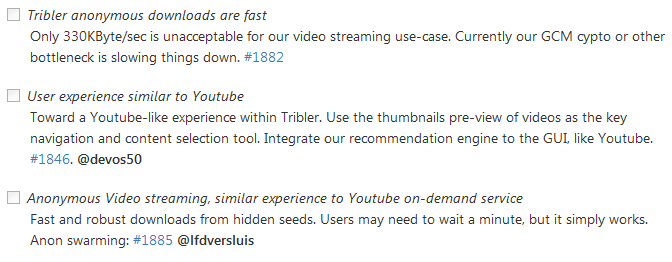
\includegraphics[width=\linewidth]{problemDescription/images/roadmap}}
	\caption{Three of the six uncompleted Tribler roadmap items.}
	\label{fig:tribler_roadmap}
\end{figure}

The Tribler project created a roadmap -- available on its GitHub repository -- to offer the same service, features, user experience, and performance as the YouTube video-on-demand service.
However, especially the poor performance of Tribler is hampering wide-spread adoption and usage. Figure~\ref{fig:tribler_roadmap} shows three of the six main uncompleted roadmap items.

\section{Key performance optimizations}

Tribler can be seen as a large and complex distributed system.
Metrics from OpenHUB show that Tribler, along with its components, features more than 169 thousand lines of code, received contributions from 111 unique contributors and took approximately 44 years of effort \cite{openhub2016tribler}.

In large and complex systems there are likely to be many performance issue present, often referred to as \emph{bottlenecks}.
J. M. Juran's Pareto principle admonishes that one should "Concentrate on the vital few, not the trivial many" \cite{ammons2004finding}. This principle is also known as the 80/20 rule.
Concretely, this means that resolving the vital bottlenecks yields the best diminishing returns, even for large systems such as Tribler.
After careful scrutiny it was decided that the most vital bottleneck to address, within the context of a nine month thesis, is Tribler's database I/O.

\section{Addressing blocking I/O}
\label{sct:triblers_database_dependency}

The problem we address within this thesis is the underlying reason for poor performance and unacceptable user experience. 
Measurements dating back from 2013 indicate that Tribler's performance is I/O-bound \cite{pouwelse2014reduce}.
Especially with slow hard disks, but also with fast SSD storage the main performance bottleneck seems to be around database access.
With our focus on the fundamental issue we believe we can make a significant step forward in making decentralized technology able to compete with centralized solutions on large-scale usage.

\begin{figure}[!h]
	\makebox[\textwidth][c]{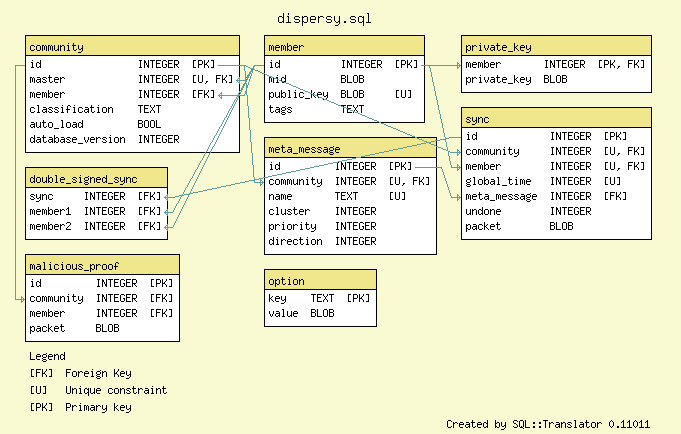
\includegraphics[width=\linewidth]{problemDescription/images/dispersy_database_schema}}
	\caption{The database schema of Dispersy, (source: Johan Pouwelse, 2013) \cite{pouwelse2013documentation}.}
	\label{fig:dispersy_database_schema}
\end{figure}

All information within Tribler is stored in a database for persistence and ease of use.
Information about the network i.e. peers, messages and authentication is stored in a separate database managed by the Distributed Permission System (Dispersy).
Dispersy is an elastic database system written in the Python programming language and uses SQLite as its underlying database engine.
It lies at the heart of Tribler, providing the means to discover peers and content in a decentralized way while offering security and anonymity.

Dispersy is fully decentralized with the exception of bootstrap servers.
It can run on systems with a large number of nodes, without any sever architecture needed \cite{dispersy2016dispersy, zeilemaker2013dispersy}.
All nodes perform the same algorithmic procedures and tasks and do not differentiate between any node i.e. all nodes are equal.

Furthermore, Dispersy provides on-to-one and one-to-many data dissemination mechanisms to forward data to nodes.
Eventually, all data will reach all nodes in the network, overcoming challenging network conditions.
The current overview of the database structure is presented in Figure~\ref{fig:dispersy_database_schema} (Johan Pouwelse, 2013).

These databases are becoming a key performance bottleneck \cite{pouwelse2014reduce}.
Back in May 2013 measurements indicated that Tribler read and wrote 660 Megabytes per hour to and from disk.
The next measurement in April 2014 showed this number was somewhat reduced to 623.
In May 2014 efforts were made to reduce this enormous amount of I/O; by batching database statements the number dropped to 538 Megabytes per hour.

So far this metric has only been measured sporadically by hand, running Tribler for an arbitrarily amount of time and check the amount of I/O by using htop\footnote{\url{http://hisham.hm/htop/}}.
htop produces an overview similar to Figure \ref{fig:iotop_tribler_april_2014} (Johan Pouwelse, 2014).
Measurements to observe to which extent Dispersy is responsible for these numbers were never conducted, however it is strongly suspected by the Tribler developers that Dispersy is responsible for most of it.
Since 2014 no work or measurements have been done related to this issue.

\begin{figure}[!h]
	\makebox[\textwidth][c]{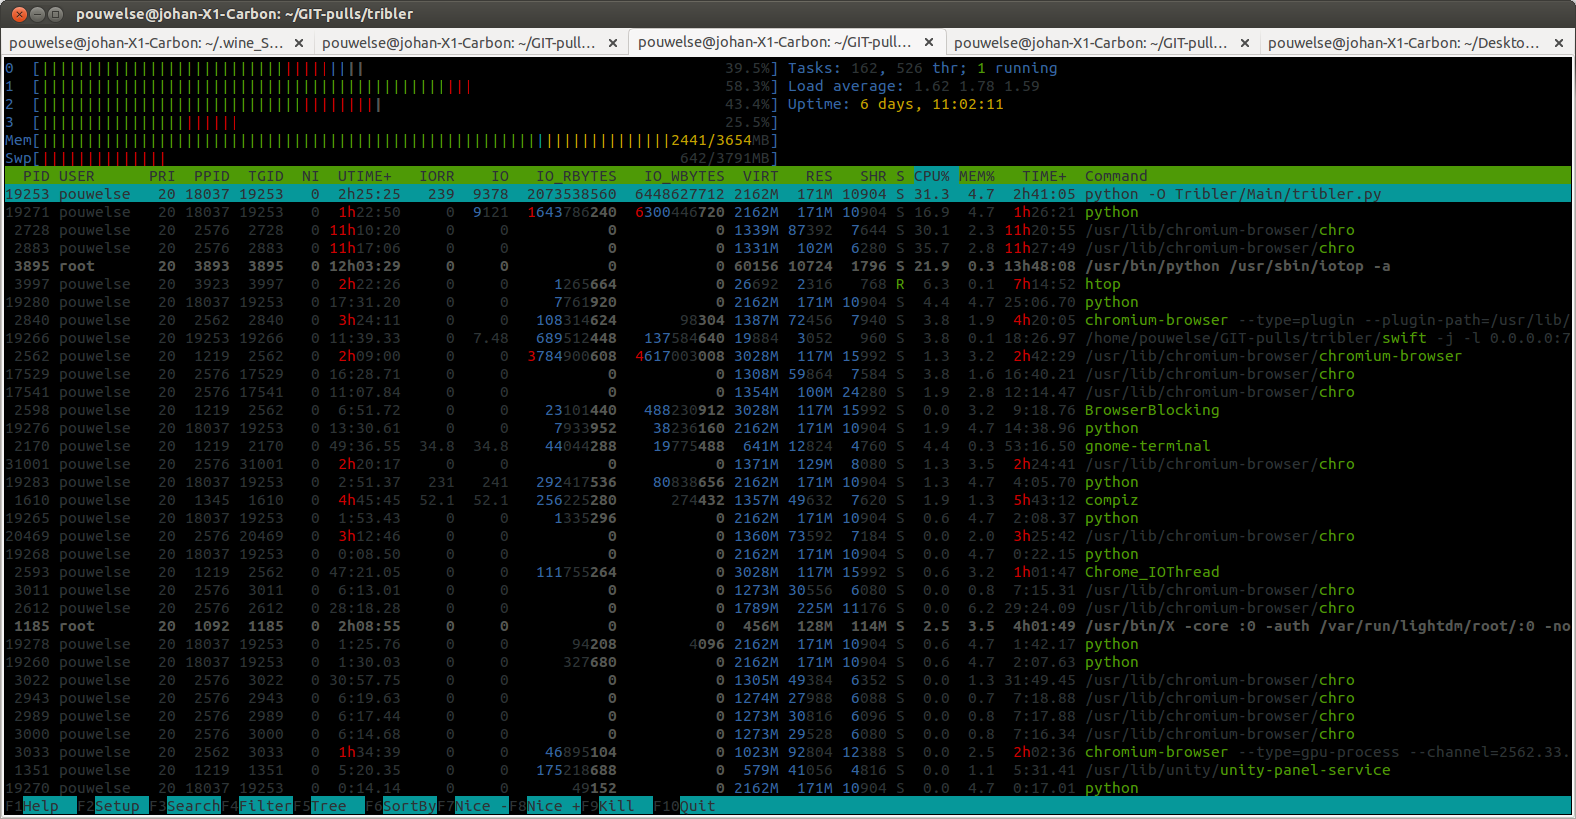
\includegraphics[width=0.9\paperwidth]{iointribler/images/iotop}}
	\caption{A screenshot of htop showing Tribler's I/O, (source: Johan Pouwelse, 2014 \cite{pouwelse2014reduce}).}
	\label{fig:iotop_tribler_april_2014}
\end{figure}

\subsection{Blocking I/O}
One of the main causes of Tribler's dramatic performance can be explained by the blocking behaviour of I/O.
Currently, Dispersy is deeply embedded into Tribler, running on the same (main) thread Tribler is running on.
Tribler, just like Dispersy, is written in the Python programming language.
In Python, a thread performing an I/O operation will block, causing all operations on the thread to suspend.
This means whenever Tribler or Dispersy performs I/O all functions of Tribler and Dispersy halt.
With the enormous amount of I/O Tribler is performing, this forms a huge limiting factor on the responsiveness and therefore performance of Tribler.

When a thread suspends, other threads can take over and perform operations, yet besides the main thread there are only two additional threads in Tribler: the Graphical User Interface (GUI) thread and the Dispersy endpoint thread.
As the name implies, the GUI is running on the GUI thread as the framework Tribler currently uses requires this.
Ironically, the Dispersy endpoint thread was introduced because of the blocking I/O behaviour.
Under heavy load, Dispersy drops packets because it cannot keep up.
Processing packets is done on the main thread and as this thread frequently blocks, the buffers overflow causing packet loss.
These two threads do not saturate the available processing time offered by the main thread blocking, leading to wasting valuable CPU cycles.

Furthermore, Tribler has seen several changes to its code base including the addition of the MultiChain: Tribler's own Blockchain-like structure \cite{norberhuis2015multichain}.
This feature heavily relies on its database to store blocks and other information about the user and other peers.
Moreover, the MultiChain makes use of its own database rather than Dispersy's.
Norberhuis points out: \enquote{The information is stored in two places within Tribler and this could be eliminated. It would reduce the disk footprint and the amount of read/write transactions as only one database would have to be maintained. The I/O ineractions are a problem according to Tribler maintainers.} \cite{norberhuis2015multichain}, yet numbers on how much I/O the MultiChain generates are not presented.
This makes it hard to estimate Tribler's current I/O rates.

Furthermore, a feature called \enquote{credit mining} is currently in development that will also interact with the database of Tribler.
There are no metrics on the current situation of Tribler and it's hard if not impossible to estimate the impact of any addition to come.
Currently, there is a lack of insight in these metrics, or a lack of \emph{software performance engineering}, causing the exact extent of the problem to be unknown.

%\section{Asynchronous I/O}
%\label{sec:async-programming}

\section{A lack of software performance engineering}

\begin{figure}[!h]
	\makebox[\textwidth][c]{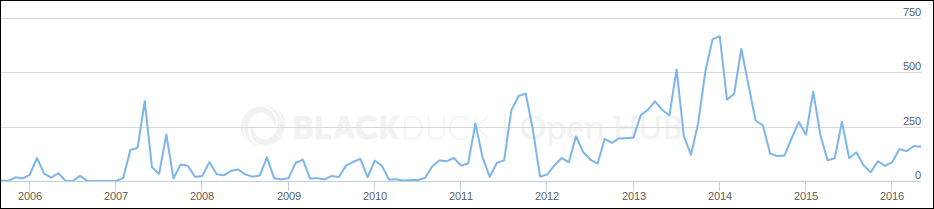
\includegraphics[width=\linewidth]{problemDescription/images/commits_openhub.png}}
	\caption{The distribution of commits on Tribler (source: OpenHUB, 2016 \cite{openhub2016tribler}).}
	\label{fig:commits_openhub}
\end{figure}

Nowadays, programs are evolving at a rapid speed and Tribler is no exception. 
Since 2005 Tribler is under continuous development, over seventeen thousands commits have been made, spanning more than a decade \cite{openhub2016tribler}.
The distribution of these commits can be seen in Figure~\ref{fig:commits_openhub}.
Code commits to fix bugs, refactor code, enhance or add functionality are pushed to code repositories at a frequent rate.
It is important that software performance engineering is a part of this process: performance should not get compromised by changes, if any it should improve.
Naturally trade-offs can be made performance wise, but it should be done with a clear understanding of the consequences.

For the past three years, attempts have been made to monitor the performance, yet with little success.
The first attempt was to create probes using Systemtap\footnote{\url{https://sourceware.org/systemtap/}}.
System tap is a tool for \enquote{instrumenting the Linux kernel for analyzing performance and functional problems}, (Jacob et al. 2008) \cite{jacob2008systemtap}.
While some success was reported, this system is no longer being maintained nor functional.
After this, code was added to the Dispersy code base to track and log if a function was running longer than a fixed amount of time.
While this implementation does provide some insight, its workings are crude and only covering some of the functions present.
For instance, it cannot handle asynchronous constructions.
Tribler did not have any observation system integrated, leaving the development team in the dark regarding its performance.

It is apparent that there is a lack of software performance engineering in the development cycle of Tribler.
Performance has never been one of the priorities in Tribler's lifetime; only 6\% of all tickets on GitHub are (indirectly) related to performance.
To ensure performance will no longer degrade realistic benchmarks need to be developed which Tribler can be tested with.
Changes can then be compared against the current codebase, tracking important performance statistics such as the amount of I/O, run time of functions, throughput and responsiveness.
These benchmarks can then be integrated into a regression testing system which can be integrated in our Jenkins continuous integration system.
Using Jenkins, performance regression tests can run on every proposed change and at predetermined moments, having a continuous updated overview of Tribler's performance metrics.

% https://github.com/Tribler/tribler/issues/15
% https://github.com/Tribler/tribler/issues/77
% experiment framework: https://github.com/Tribler/tribler/issues/114
% latency grpahs? https://github.com/Tribler/tribler/issues/119
% speed of streaming: https://github.com/Tribler/tribler/issues/134
% of course: https://github.com/Tribler/tribler/issues/3
% nightly runs: https://github.com/Tribler/tribler/issues/184
% extreme cpu ticket: https://github.com/Tribler/tribler/issues/197
% slow startup time ticket: https://github.com/Tribler/tribler/issues/255

\section{Realistic benchmarks}
Directly related to the performance problem is the benchmark problem.
In order to improve user performance we require making assumptions about realistic use cases.
Each user has different usage patterns, hardware and network conditions, all affecting performance.
Creating one of more several benchmarks testing several scenario's is required to accurately tune the system for real world usage.
At the same time, a benchmark cannot consume too much time.
Benchmarking is by nature time consuming \cite{huang2014performance}, however running long regression tests per commit done on a pull request will severely strain the development speed.

Therefore, it is important to create a reference benchmark which has a close resemblance to real world usage without consuming too much time.

The next step is to introduce a solution, tracking changes in vital numbers such as CPU consumption or I/O produced.
Any improvement indicated by this benchmark should reflect improvement for real world users.
This system should benchmark the current code base against proposed changes, capturing any differences in performance.


%\section{OLD TEXT}
%Only by comparing different builds can one gain insight into performance changes.
%Currently Tribler lacks this insight.
%As Tribler is heavy I/O-based and likely I/O-bound, it is crucial to have these numbers.
%A breakdown of database statements is needed and the amount of I/O that is generated.
%Recently a block-chain like structure called the Multi-Chain was added to Tribler and soon another feature called credit mining will be introduced as well.
%The impact and increase of I/O caused by these additions are unknown.

%Ideally, we would like to run regression tests on multiple platforms powered by our Jenkins continuous integration system as visualized by Figure X \todo{make figure.}.
%This regression test will feature average use cases and automatic graph generation to give developers an instant overview of their changes.
%This system has to run automatically whenever a pull request is opened on GitHub.
%Efforts can then be made to optimize the I/O output and improve the performance of Tribler.

%\section{Resolving bottlenecks}
%To improve the performance of Tribler, (I/O) bottlenecks to need to be removed.
%The key problem here is how to identify and resolve bottlenecks in a complex system such as Tribler.

%By careful inspection of the usage of I/O, we identified that Tribler's I/O is blocking the main thread.
%Many programming languages have support for parallelization, allowing multiple functions to be executed at the same time by using threads.
%Tribler does not have access to this paradigm as it's written in the Python programming language.
%Python lacks this feature as only one thread can run in the Python interpreter at any time because of the Global Interpreter Lock (GIL).
%However, a thread does release the GIL when it's performing a blocking I/O operation, allowing other threads to get a hold of the GIL and run.
%Leveraging this trait to gain performance is a huge step forward towards solving the (I/O) bottleneck Tribler is currently facing.

%\section{Tribler's code base}
%At the same time, Tribler's current code base has a severe lack of (unit) tests, structure and documentation and contains dead code.
%The current version has been in development for over nine months, is plagued with bugs and non-functioning on some platforms.
%As of writing, the code is only tested on a single Unix operating system.
%Tribler, however, is available for all three major operating systems: Windows, Mac OS and Unix distributions.
%As users are reporting platform specific bugs, it is evidently important that automated testing on all three platforms are realized.
%All this results in long and complex debugging processes and creates a steep learning curve for new students joining the project and might withhold members of the open-source community to start contributing.

%While it's not this thesis primary goal, refactoring the code involved with the bottlenecks and properly documenting and testing %this refactored code is a secondary goal of this thesis, aiding in lowering the learning curve and improving the stability of %the Tribler code base.

% \section{Connectability}
% One of the problems Tribler faces is the connectability of its users.
% Users can be behind e.g. firewalls that prevent incoming or outgoing connections.
% Currently, Tribler employs NAT and Firewall Traversal [CITE], yet the success of this method is limited.
%The Tribler team has implemented their own Distributed Hash Table (DHT) in python while existing libraries such as LibTorrent also offer these.
% These implementations should be tested to see if changing to a library offers a significant boost in terms of exchange or speed.

%When users are downloading anonymously, they are inside so-called `hidden swarms'.
%These hidden swarms are not present in e.g. LibTorrent's DHT and therefore information from peers has to be exchanged between peers themselves by means of introducing peers to each other (PEX).
%By making use of Dispersy, Tribler creates rendezvous points to introduce peers to each other.
%If these rendezvous points are not connectible, PEX cannot take place.
%Solving this may be done by always connecting to the same port (chosen by the user or a default) and ask the user to forward that port.
%If users are not willing to do so, they can be penalized.
%This penalty can be for example not able to download anonymously at all, receive half the amount of credits when credit mining (see [CITE]) or limited download speed.

% \section{Anonymous download speed}
% To allow for anonymous downloading, Tribler uses a Tor-like technique to create so called `anon tunnels'.
% To increase download speed and prevent a bottleneck in the network hampering the overall download speed, several tunnels are built to download simultaneously from [CITE?].
% Since this Tor-like technique includes cryptographic functions, having multiple tunnels running concurrently results in a lot of cryptographic calls being executed.
% Stok et al. profiled Tribler using a gumby\footnote{Gumby is Tribler's experiment running framework.} experiment. This experiment showed that a lot of processing time is spent on encrypting and decrypting packets [CITE] as well as serializing and deserializing data.
% Currently, the CPU power is a bottleneck when downloading using the anonymous tunnels.
% By offloading the encryption and decryption of packets to a separate core, the workload on the core on which Tribler is running can be reduced.
% This should yield an increased download speed and better spread of workload overall as more packets can be processed per time unit.

% \section{Package serialization}
% One of the core components of Tribler is Dispersy. 
% Dispersy is a fully decentralized elastic database capable of communicating packets and exchanging peers.
% Both Dispersy and Tribler make use of python' built-in serialization function.
% The profile ran by Stok et al. [CITE] indicated that a significant amount of CPU resources is spent on serializing data when sending or receiving UDP packets.
% As previously explained, running multiple threads at once does not result in code being executed concurrently.
% Cap'n Proto is a serialization framework that offloads the serialization of packets to a C++ process, which bypasses the global interpreter lock.
% This means that the other threads -- who are still affected by the global interpreter lock -- can immediately continue their work as the locks is released once the offloading to the C++ code base is done.

% \section{Responsiveness}
% Since Tribler is written in the python language, calls on any thread will cause other threads to halt their execution. % this is wrong.
% Normally two separate threads can run code in parallel as they generally do not touch each other's state.
% The cause of this is the Global Interpreter Lock (GIL) which states that only one function can be executed at a time.
% In its current state, the Graphical User Interface (GUI) of Tribler will block if it's doing some CPU or I/O intensive work.
% This yields a scenario in which the user is unable to perform any action, which is not user friendly.
% In some cases the operating system itself will show e.g. a warning or visualisation that the process is not responding.
% To solve this issue, heavy operations should be done on separate threads or processes which are not monitored by the GIL.
% Several libraries that are written in C/C++ are a good example of this.
% Once the code of such a library is invoked and the execution is offloaded to the C/C++ code, the GIl is released, allowing other python code to ran in parallel.
% Another approach is using the python framework Twisted.
% Twisted has implemented a thread pool that also bypasses this GIL.
% By rewriting CPU or I/O intensive code to make use of this thread pool in an asynchronous way, the responsiveness of Tribler can be improved.

% \section{Code quality and testing}
% Tribler's current code base is in a bare state.
% The current version that has been in development for over nine months now is plagued with bugs and is non-functioning.
% Furthermore, there is a severe lack of unit tests, a lot of the code is undocumented and unnecessary complex and structure and flow are missing.
% This results in long and complex debugging processes when bugs are found and raise the bar for new contributors to get familiar with the code base.

% As of writing, the code is only tested on a single Unix operating system.
% Tribler, however, is available for all three major operating systems: Windows, Mac OS and Unix distributions.
% As users are reporting platform specific bugs, it is evidently important that automated testing on all three platforms are realized.

% Refactoring the code is necessary in order to regain the structure and lower the code complexity.
% Furthermore, proper unit tests are required to ensure Tribler's stability now and in the future.
% These tests have to be executed on build machines that run different operating systems, preferably with various configurations e.g. 32 and 64 bit architectures or different library versions.

\section{Objective and research questions}
\label{chp2:sct:objectives-research-questions}
The objective of this thesis is to improve the performance and responsiveness of Tribler and to introduce a regression test system.
The verification of the performance regression test system is done by focussing on removing Tribler's biggest bottleneck present: blocking database I/O.
By resolving this bottleneck, important metrics tracked by this regression test system should show positive changes, indicating improvement.
%In general, projects facing similar issues can adopt the practices applied when changes made to the Tribler code base.\\

The research presented in this thesis was carried out in cooperation with the Tribler team. 
The Tribler team consists of both staff members of the Technical University of Delft as well as Bachelor and Master students.
Based on the objectives of Tribler, this thesis aims to answer the main research question formulated below.\\

\textbf{Main Research Question:} How can we improve Tribler's performance, responsiveness and throughput?\\

To answer this main research question, we have defined three research questions below. Each of these research questions will be justified as why they contribute to the main research question.\\

\textbf{Research Question 1:} Can a system such as Tribler benefit from asynchrony?\\

To improve performance and responsiveness, parts of Tribler can be rewritten to become asynchronous.
By performing tasks asynchronously the performance and responsiveness of a program can improve.
However, an asynchronous approach can have its drawbacks. 
One of these drawbacks is that it requires a different mindset for the programmers as the whole call chain and structure of a program becomes different.
Identifying these drawbacks and deciding if the benefits outweigh the costs is necessary to prevent the current state from worsening. \\

\noindent
\textbf{Research Question 2:} How do we incorporate software performance engineering into Tribler to gain insight into performance statistics?\\

Currently, not a single developer has insight into how well Tribler performs and what impact changes have on Tribler in its current state.
To be able to conclude performance changes do not negatively impact the performance of Tribler, we can apply software performance engineering.
Software performance engineering focuses on introducing performance regression tests and benchmarks into the development cycle.
By making use of these regression tests, Tribler developers finally get insight into vital metrics which are desperately needed.\\

\textbf{Research Question 3:} How do we create benchmarks which are a representative use case of Tribler?\\

Ultimately, the end user should benefit from performance enhancements.
The key issue here is to define metrics and workloads to benchmark with.
Metrics need to properly capture changes to accurately measure the impact of any modification.
Additionally, if the workload does not represent a realistic use-case the benchmark may be flawed, rendering the outcome unreliable and inaccurate.

A second constraint is the run time of a benchmark.
Preferably, the regression testing system should not clog the throughput of the current test architecture.
Running an one hour benchmark per change per pull request will severely strain the development speed.

\section{Main contributions}
The main contributions of this thesis are as follows.
First, we elaborate on the subject of multitasking and parallelization in the context of the Python programming language and provide arguments where asynchronous programming is preferred over synchronous programming, using Tribler as a case study.
We then resolve the vital I/O bottleneck currently present in Tribler using asynchrony and a multi-threaded approach.
This is done by introducing the Storm database framework into Tribler and creating a database manager with an asynchronous, non-blocking yet serialized interface.
Next, we introduce software performance engineering into Tribler's development process by adding a regression testing system that benchmarks different versions of the same code base to gain insight into performance metrics such as disk I/O.
Finally, experimental results and measurements will be provided to confirm the main goal of this thesis i.e. improving responsiveness, performance and user experience.

%Related work
%\chapter{Related work}

\section{Parallelism and asynchrony in Python}
\label{sct:parallelism_and_asynchrony_in_python}
Parallelize Python by removing the GIL, introducing asynchronous behaviour or by other means is a topic that regularly returns in e.g. the Python mailing list, topics as PyCon and other events \cite{python2015global}.
To gain performance, many attempts have been made to alter Python or remove the GIL to fully benefit from multiple CPU's.
To date, no one has ever succeeded in removing the GIL and meet the (hard) requirements for replacement \cite{python2015global}.

On of the most well-known alternative implementations of Python is PyPy.
It makes use of a tracing Just-in-Time compiler to produce optimized code \cite{bolz2009tracing}.
By doing so, PyPy offers increased speed, reduced memory usage and support for stackless mode while providing a highly compatibility with existing python code \cite{pypy2016pypy}.
PyPy's geometric average is 7.6 times faster than CPython (normal Python) \cite{pypy2016speed}.
While it has many popular libraries ported to be used with Pypy, it still lacks some common used packages.
Moreover, most of these libraries are not available on the official packaging repositories of Ubuntu and/or Debian.

Two other popular implementations are JPython and IronPython.
Both of these projects have removed the GIL and can fully exploit multiprocessor systems \cite{python2015global}.

JPython is a Python interpreter implemented in Java. It can be integrated in Java applications and allows python applications to be compiled into Java classes.
Using JPython, Python after compiled to java bytecode will run in the Jython virtual machine, giving full access to all Java APIs and classes \cite{jython2016why}.

IronPython does basically the same as JPython, compiling the source to in-memory bytecode and runs it on the Dynamic Language Runtime \cite{ironpython2014}.
It allows developers to run Python using the .NET framework.

To illustrate the attempts to remove the GIL are still on going, Larry Hastings presented ``The Gilectomy'' at PyCon 2016.
He showed that removing the GIL is fairly easy, but has a huge negative impact on CPython's performance.
Additionally, he explained the reason why this performance loss was observed and names some methods that may make ``The Gilectomy'' a viable alternative to CPython.\\

Libraries and frameworks that introduce asynchrony are also available in large numbers.
In particular, many projects exist that attempt to make I/O asynchronous \cite{asyncio2016python}.

Twisted is an event-driven networking engine written in Python.
It allows for event-driven and asynchronous programming using deferreds.
Twisted has a custom event-loop called the reactor, on which tasks can be scheduled.
This reactor handles callbacks/errbacks fired by deferreds and contains many utility functions and classes to perform asynchronous and non-blocking calls.
Unlike many libraries and frameworks available, Twisted is available on the official repositories of Ubuntu and Debian and is a well tested, mature framework.

In 2012 Guido van Rossum embarked on a journey to add asynchronous I/O to the Python 3 standard library.
The asyncore library is showing it's age and according van Rossum \enquote{We have to throw it away and forget it ever existed.} (Guido van Rossum, PyCon 2013).
Van Rossum wrote a new Python Enhancement Proposal (PEP)\footnote{https://www.python.org/dev/peps/pep-3156/} and implemented a new framework \enquote{Tulip} \cite{edge2013pycon}.
Tulip's implementation and features are inspired by many well-known asynchronous frameworks such as Twisted and Tornado.
Tulip features Coroutines, Futures and Tasks.
Coroutines are equivalent to callbacks which are python generators under the hood.
Futures are similar to deferreds in Twisted, which is a placeholder for a value that is currently being computed.
Tasks are Futures wrapped in Coroutines.
Just like Twisted, Tulip features an event loop which multiplexes different activities such as callbacks and signals. 
It was added to Python 3.3 and is now part of the Python standard library in Python 3.4.
There are no plans to make Tulip available for older Python versions such as 2.7 or 3.2.

Decorated Concurrency (DECO) uses the multiprocessing package of Python to parallelize functions using a ``concurrent'' decorator \cite{sherman2016deco}.
Different processes have their own GIL, which allows for parallel processing.
Similarly, the ``synchronized''  inserts synchronization events to automatically refactors assignments of the results of ``concurrent'' function calls to happen during synchronization events.
However, because of the overhead of creating a new process and communicating between different processes, this approach is only viable for heavy loads that generally can run on its own and requires heavy computation.

\section{Regression testing}
Regression testing has been extensively studied both in research as industrial appliances.
\todo{Add related work regarding regression testing.}

\section{Profilers}
Resolving bottlenecks using profilers has been applied for many years: \cite{pesterev2010locating, gorelick2014high, fan2013performance}.
By default, Python ships three profilers:

\begin{enumerate}
	\item cProfile is a C extension that has reasonable overhead. It is the current recommended profiler. It provides the same interface as the ``profiler'' profiler.
	\item profiler is a profiler written in pure Python. It adds a lot of overhead and its usage is discouraged. However, because it's written in Python, it does allow for easier extension than it's C counterpart cProfile.
	\item hotshot was an experimental C module which is now deprecated as its no longer maintained. While it's still present, the module may be dropped in a future version of Python.
\end{enumerate}

Alternatively, profilers have been developed by the open-source community.
Yappi is a profiler written in the C language that is thread-aware, allowing automatic profiling of multi-threaded applications [CITE]\todo{cite}.
It provides options to measure CPU or wall time, sort the output by various parameters and support the callgrind and pstat output formats.

Savrun-Yeni{\c{c}}eri et al. introduced an event-based profiler that performs better than the Python standard profilers which requires modest implementation effort \cite{savrun2015efficient}.
Their profiler helps users find bottlenecks in programs, aids language implementers to improve the performance of their language implementation and allows the comparison and evaluation of different languages using cross-language benchmarks.\\

% Python's threading model
\chapter{Python's threading model}
\label{cpt:pythons_thread_model}

Before we can address Tribler's blocking I/O problem, we first need to better understand Python's threading model and how the Python interpreter behaves.
By looking in depth how the operating system (OS) and the python interpreter behave together, how threads run concurrently and the pros and cons of concurrency, we can look into if asynchrony can boost Tribler's performance.
This allows us to answer the second research question \enquote{Can a system such as Tribler benefit from asynchrony?} and gives us a direction of design and implementation.

\section{Threads in Python}

\begin{figure}[!h]
	\makebox[\textwidth][c]{\includegraphics[width=\linewidth]{pythonthreading/diagrams/thread_io_release_diagram}}
	\caption{A schematic view of how threads release the GIL when performing IO in Python.}
	\label{fig:python_threads_release_gil}
\end{figure}

Python threads are normal OS threads, either POSIX (pthread) or Windows threads \cite{beazley2010understanding, beazley2009inside}.
Python does not feature a thread scheduler, threads are fully managed by the operating system that hosts them.
To control thread execution Python features a construct called the Global Interpreter Lock (GIL).
This GIL ensures that only one thread can run in the python interpreter at once, i.e. a thread needs to hold the GIL in order to execute.
This means there cannot be any parallel execution.
Once a thread is done executing or needs to block it releases the GIL.
This gives way for cooperative multitasking as other threads that are ready to execute can try to acquire the GIL, visualized in Figure \ref{fig:python_threads_release_gil}.

To make sure Central Processing Unit (CPU) bound tasks do not hold the GIL indefinitely a simple check mechanism is built in that \enquote{checks} every thread once per 100 ticks.
Ticks are loosely mapped to interpreter instructions and do not define a time unit.
Listing \ref{lst:one_tick} contains two code samples that only take one tick each, but take require different amount of time to compute.

\lstinputlisting[caption={Two code samples that each take one tick yet require a different amount to compute.},label={lst:one_tick},language=Python]{pythonthreading/code/one_tick.py}

When a check is run the following four steps are executed:
\begin{enumerate}
	\item The thread that holds the GIL resets its tick counter.
	\item If the current thread it the main thread, it runs the signal handlers.
	\item The thread releases the GIL.
	\item The thread tries to reacquire the GIL.
\end{enumerate}

Note that a thread may immediately reacquire the GIL after releasing it.
Since every thread has this check, CPU-bound threads will engage in cooperative multitasking.

\section{Multi threaded programming performance}
\label{sct:multi_theaded_programming_performance}

\begin{table}[h]
	\centering
	\begin{tabular}{l|l}
		\textbf{Component} 	& \textbf{Specifications} \\ \hline
		Operating System   	& Ubuntu 16.04 LTS \\
		Python version		& 2.7.12 \\
		CPU					& Intel Core i5-2410M \\ 
		HDD					& Samsung 850 EVO 250GB  \\ 
		RAM					& 8 GB DDR3 1600MHz \\
	\end{tabular}
	\caption{Specifications of the setup used during the rerun David Beazly's experiment.}
	\label{table:rerun_beazily}
\end{table}

Because threads cannot run in parallel, this changes the performance one may expect from a multi-threaded program.
Dadiv Beazly presented his findings in his Python Concurrency Workshop (2009) \cite{beazley2009inside}.
By running a trivial CPU-bound function using two threads on a dual-core MacBook, processing time increased 24.6 to 45.5 seconds; an increase of 185\%.
Disabling one of his cpu cores yielded 38.0 seconds, an increase of 154\% in run time.

To confirm this behaviour still exists in the latest version of Python2, we rerun Beazly's experiment.
The setup used in this experiment can be found in Table~\ref{table:rerun_beazily}.
Running it sequentially gives us a run time of 8.17 seconds, whereas running it using two threads provides us with a run time of 14.49 seconds; an increase of 177\% which is in range of Beazley's observations

To investigate this behaviour, Beazley studied the underlying C code to inspect why he was observing these performance results.
Whenever a (Python) thread releases the GIL, it sends out a signal.
The OS then propagates this signal to other threads which then can attempt to acquire the GIL.
The time or \emph{lag} between thread switching and execution may be significant depending on the OS, according Beazley.
Most operating systems make use of a priority system for threads: the thread with the highest priority will be scheduled by the OS.
Often, CPU-bound threads have a low priority and I/O-bound threads a high priority.
If a signal is send to a low priority thread and all CPUs are currently busy processing other, high priority threads, it won't be run until one of the CPUs becomes available.

As it turns out, the GIL signalling is the source of the performance loss.
Whenever the periodic \enquote{check} runs, the following happens:

\begin{itemize}
	\item First the Python interpreter locks a mutex.
	\item Next, it signals on a condition variable/semaphore where another thread is \emph{always} awaiting execution.
	\item Because of this waiting thread, additional pthread processing and system calls are generated to deliver the signal.
\end{itemize}

Beazley provided rough measurements on the number of system calls generated, summarized in Table~\ref{tbl:system_calls_thread_switching}.
From these numbers Beazley concludes that the amount of additional calls generated is significant and the main reason for the performance loss.
He then dived deeper into these numbers to find a cause.

 \begin{figure}[h]
 	\makebox[\textwidth][c]{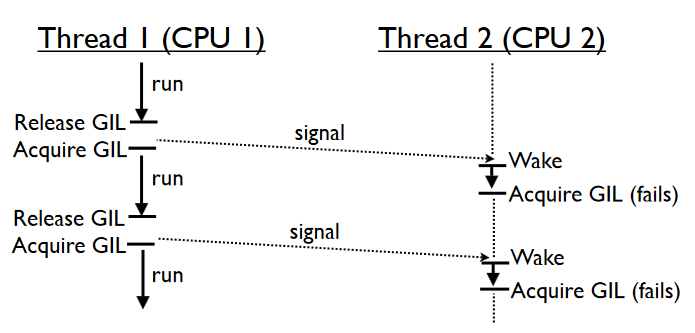
\includegraphics[width=\linewidth]{pythonthreading/images/gil_battle_threads}}
 	\caption{A schematic view of two threads battling for GIL acquisition (source: David Beazley, 2009).}
 	\label{fig:gil_battle_threads}
 \end{figure}

By recording a real-time trace of all GIL related operations i.e. acquisition, release, etc., Beazley was able to reconstruct the key problem.
When running multiple CPU-bound threads on multiple cores, all of them will be scheduled \emph{simultaneously}.
The threads proceed to battle over GIL acquisition. 
Whenever a thread releases the GIL because of the 100 tick \enquote{check}, it immediately tries to reacquire it.
Another thread will also try to acquire the GIL upon this signal, but as this signal arrives with a delay it will most likely fail.
This processes is visualized by Figure~\ref{fig:gil_battle_threads} (David Beazley, 2009).
Beazley argues that here two competing goals are clashing.
On the one hand Python wants to only run one thread at a time where on the other hand the OS wants to schedule as many processes/threads to take advantage of its multiple core architecture.
This clash raises a lot of overhead, which results in a severe performance penalty.

Even running threads on one core result in these GIL acquisition battles.
I/O-bound threads which are high priority may fail to acquire the GIL when a CPU-bound thread is busy, degrading the response time of the I/O thread.

\begin{table}[]
	\centering
	\caption{A summary of the measurements from David Beazley \cite{beazley2009inside}.}
	\label{tbl:system_calls_thread_switching}
	\begin{tabular}{|l|l|l|l|}
		\hline
	\textbf{Threads}	& \textbf{Cores} & \textbf{Unix system calls} & \textbf{Mach system calls} \\ \hline
	1	& 1 & 736 & 117 \\ \hline
	2	& 1 & 1149 & 3.3M \\ \hline
	2	& 2 & 1149 & 9.5M \\ \hline
	\end{tabular}
\end{table}

\subsection{A new GIL}

To solve the excessive amount of GIL signalling, a new GIL has been introduced in Python 3.2 \cite{beazley2010understanding}.
Instead of having the 100 ticks \enquote{check}, there is now a global variable.
A thread will continue running until this variable is set to one (1), indicating another thread requests to acquire the GIL at which the running thread must release the GIL.
This means whenever only one thread is running, the variable will never be set (there is no competing thread) and no signalling takes place.
Whenever another thread is present, it will be in a suspended state as it does not hold the GIL, and starts a five millisecond timeout.
From here two things can happen: the running thread releases the GIL voluntarily within the timeout (e.g. an I/O operation is performed) at which the other thread can immediately acquire it, or the timeout expires.
If the timeout expires, the other thread will set the global variable to one and enters another timeout, awaiting a signal that the GIL has been released.
The running thread will release the GIL, sends out a signal that it has done so and starts a wait period.
When the other thread acquires the GIL it will send out an acknowledgement to the thread that just released the GIL and starts its computations.
Finally, the former running thread will now enter a timeout upon receiving the acknowledgement so that it may require the GIL again.

To observe if the new GIL has any better performance, Beazley ran the same experiment using Python 3.2 and the results look promising.
Running the code sequentially, using two threads and using four threads on a quad core MacBook resulted in run times of 11.53, 11.93 and 12.32 second respectively.
Unfortunately, there are caveats when performing I/O operations using the new GIL.
Whenever an I/O operation does not block, the thread still releases the GIL which requires the thread to initiate the timeout again to reacquire the GIL.
Meanwhile CPU bound threads will also attempt to acquire the GIL since it was released, causing stalls.
Beazley argues that some more work is required on the GIL to get rid of this behaviour, yet expresses that even with the GIL present threads can still deliver excellent performance and programmers still should use threads when appropriate.

Unfortunately, Tribler currently runs on Python 2.7 and a considerable amount of work is required to migrate to Python3.
However, as the new GIL does look promising with respect to blocking I/O it can be noted down as an item for future work.

\section{Attempts to parallelize Python}
\label{sct:removing_the_gil}

Parallelize Python by removing the GIL and other means to speed up Python are topics that regularly return in the Python mailing list and at PyCon \cite{python2015global}.
Throughout the years many attempts have been made to alter Python or remove the GIL to fully benefit from multiple CPUs.
To date, no one has succeeded in removing the GIL and meet the (hard) requirements for replacement \cite{python2015global}.

On of the most well-known alternative implementations of Python is PyPy.
It makes use of a tracing Just-in-Time compiler to produce optimized code \cite{bolz2009tracing}.
By doing so, PyPy offers increased speed, reduced memory usage and support for stackless mode while providing a high compatibility with existing python code \cite{pypy2016pypy}.
PyPy's geometric average is 7.6 times faster than CPython (normal Python) \cite{pypy2016speed}.
While it has many popular libraries ported to be used with PyPy, it still lacks some common used packages.
Moreover, most of these libraries are not available on the official packaging repositories of Ubuntu and/or Debian, rendering PyPy unusable for the Tribler project as publishing Tribler on said repositories requires the dependencies to be available on them as well.

Two other popular implementations are JPython and IronPython.
Both these projects have removed the GIL and can fully exploit multiprocessor systems \cite{python2015global}.

JPython is a Python interpreter implemented in Java. It can be integrated in Java applications and allows python applications to be compiled into Java classes.
Using JPython, Python after compiled to java bytecode will run in the Jython virtual machine, giving full access to all Java APIs and classes \cite{jython2016why}.

IronPython does basically the same as JPython, compiling the source to in-memory bytecode and runs it on the Dynamic Language Runtime \cite{ironpython2014}.
It allows developers to run Python using the .NET framework.

To illustrate the attempts to remove the GIL are still on going, Larry Hastings presented \enquote{The Gilectomy} at PyCon 2016.
He showed that removing the GIL is fairly easy, but has a huge negative impact on CPython's performance, cache misses being the main reason.
Additionally, Hastings names some methods that may make The Gilectomy a viable alternative to CPython.\\

Libraries that introduce parallelism or asynchrony to gain performance are also available in large numbers.
In particular, many projects exist that attempt to make I/O asynchronous \cite{asyncio2016python}.
Often, these leverage the multiprocessing package in the standard library of Python.

Decorated Concurrency (DECO) uses the multiprocessing package of Python to parallelize functions using a \enquote{concurrent} decorator \cite{sherman2016deco}.
Different processes have their own Python interpreter which in turn has its own GIL, which allows for parallel processing.
Using the \enquote{concurrent} decorator, a function will be wrapped and executed on a new process.
Similarly, the \enquote{synchronized}  inserts synchronization events to automatically refactor assignments of the results of \enquote{concurrent} function calls to happen during synchronization events.
However, because of the overhead creating a new process generates and communicating between different processes, this approach is only viable for heavy loads that generally can run on its own.
The authors mention that a function should at least have an execution time of one millisecond for this method to be beneficial.

\section{Asynchronous programming}

\begin{figure}[!h]
	\makebox[\textwidth][c]{\includegraphics[width=0.6\linewidth]{pythonthreading/diagrams/normal_execution_flow}}
	\caption{Synchronous processing of tasks}
	\label{fig:normal_execution_flow}
\end{figure}

\begin{figure}[h]
	\makebox[\textwidth][c]{\includegraphics[width=0.6\linewidth]{pythonthreading/diagrams/delays_in_execution}}
	\caption{Tasks will be waiting when disk or network has to catch up.}
	\label{fig:delays_in_execution}
\end{figure}

A second option it to make use of asynchronous programming to gain performance.
Traditionally, synchronous programs execute tasks one by one as visualized in Figure\ref{fig:normal_execution_flow}.
When these functions perform an I/O operation, they are waiting for the disk or network to catch up, visualized in Figure~\ref{fig:delays_in_execution}.
In turn, the thread these functions run on will block, see Figure~\ref{fig:normal_io_flow}.
This means the main thread of a program will block if the I/O call happens on that thread.
A synchronous program that performs I/O operations regularly will therefore spend much of its time blocked waiting for disk or network to catch up.

\begin{figure}[t]
	\centering
	\begin{subfigure}[b]{\textwidth}
		\includegraphics[width=\textwidth]{problemDescription/images/normal_io_flow.png}
		\caption{A schematic overview of an I/O operation done by the main thread (synchronous).}
		\label{fig:normal_io_flow}
	\end{subfigure}
	~ %add desired spacing between images, e. g. ~, \quad, \qquad, \hfill etc. 
	%(or a blank line to force the subfigure onto a new line)
	\begin{subfigure}[b]{\textwidth}
		% To not scale this picture, the width of the normal flow image is 755, this one 595, hence a ratio of 0.79
		\includegraphics[width=0.79\textwidth]{problemDescription/images/async_io_flow.png}
		\caption{A schematic overview of an I/O operation executing on a separate thread, retuning a deferred (asynchronous).}
		\label{fig:async_io_flow}
	\end{subfigure}
	\caption{A schematic overview of a how an I/O call is handled in a synchronous versus an asynchronous manner.}
\end{figure}

In asynchronous programming, tasks are split into multiple chunks and executed interleaved, see Figure~.
The fundamental idea behind this approach is that when faced with a task that would normally block waiting for I/O, it will instead execute some other task that can still make progress.
This approach can outperform a synchronous program dramatically.

Support for asynchrony in python 2.7 is poor so the use of a framework is required.
Tribler makes use of Twisted, an event-driven networking engine written in Python which allows for event-driven and asynchronous programming \cite{kinder2005event}. 

When programming asynchronously in Twisted, the function that is being called (callee) returns a deferred.
A deferred is a place holder for the actual value that the callee eventually will return once its done computing.

To ensure I/O operations does not block the main thread, the I/O can be moved to a separate thread, returning a deferred.
By attaching a callback and an errback, the caller can handle the case of a success and failure respectively.
These callbacks are handled by Twisted's event loop.
This thread can then block while the main thread continues executing other scheduled task.
Once the thread is done with its task it can invoke the callback of the deferred, notifying Twisted's event loop.
The event loop will then schedule the continuation of the previous task and proceeds executing the current task if not done yet, see Figure~\ref{fig:async_io_flow}.

\subsection{Drawbacks}

The main drawback of asynchronous programming is that it makes the structure and execution of a program more complex.
As any task can run while another task is blocking, one must be careful that the current task does not modify information the blocking task is dependant on.
Especially when working with databases one needs to make sure that the order of database queries is not different.

A second point of attention is the overhead generated when creating multiple threads.
As pointed out by the previous sections, offloading work to multiple threads may actually have a negative impact on performance.

\subsection{Initial measurements}

\begin{table}[h]
	\centering
	\caption{Specifications of the setup used in the initial CPU/IO/Network experiment}
	\label{table:setup_initial_experiment}
	\begin{tabular}{l|l}
		\textbf{Component} 	& \textbf{Specifications} \\ \hline
		Operating System   	& Ubuntu 15.10 \\
		Python version		& 2.7.11 \\
		CPU					& Intel Core i7-2630QM \\ 
		HDD					& Samsung 850 EVO 500GB  \\ 
		RAM					& 8 GB DDR3 1600MHz \\
	\end{tabular}
\end{table}

\begin{table}[]
	\centering
	\caption{Overview of which workload is processed asynchronously per run configuration.}
	\label{tbl:experiment_configuration}
	\begin{tabular}{|c|c|c|c|}
		\hline
		\textbf{Configuration}	& \textbf{I/O Asynchronous} & \textbf{CPU Asynchronous} & \textbf{Network Asynchronous} \\ \hline
		0	& no & no & no \\ \hline
		1	& yes & no & no \\ \hline
		2	& no & no & yes \\ \hline
		3	& yes & no & yes \\ \hline
		4	& no & yes & no \\ \hline
		5	& yes & yes & no \\ \hline
		6	& no & yes & yes \\ \hline
		7	& yes & yes & yes \\ \hline
	\end{tabular}
\end{table}

\begin{figure}[h]
	\makebox[\textwidth][c]{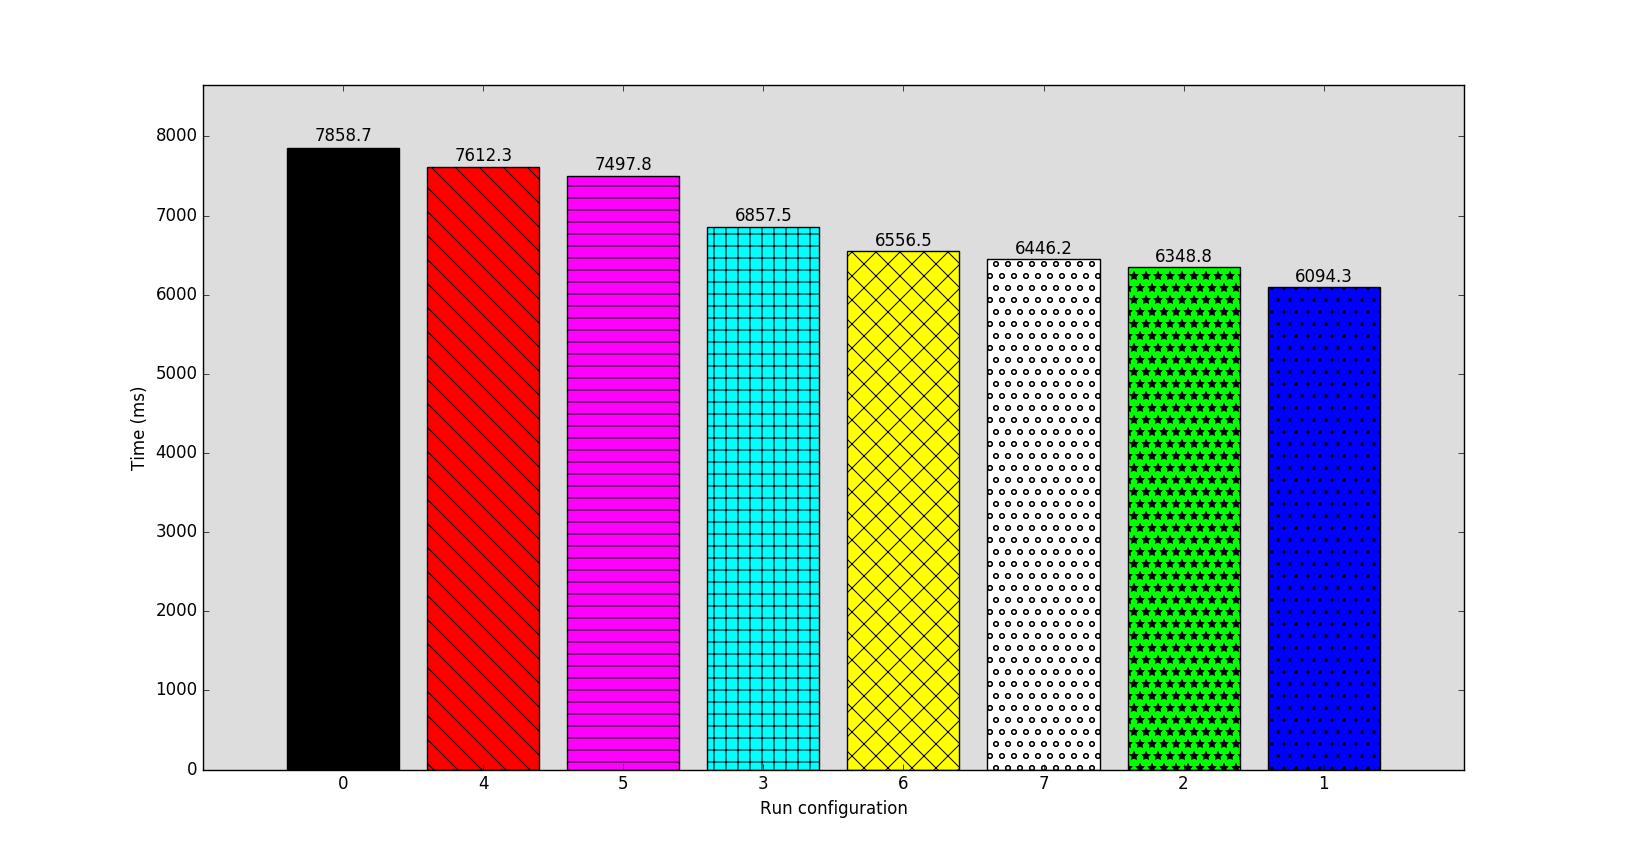
\includegraphics[width=0.9\paperwidth]{pythonthreading/images/initial_async_results}}
	\caption{Results of the initial experiment.}
	\label{fig:initial_results}
\end{figure}

To observe if Tribler can benefit from asynchrony, an experiment has been conducted which replicates Tribler's workload.
An overview of the system this experiment is available in Table~\ref{table:setup_initial_experiment}.
As Tribler functions as both a client and a server, CPU, I/O and network tasks are run interchangeably.
To mimic these workloads, the experiment has been set up as follows. 

First, as Tribler is both a client and a server, six client-server pairs are constructed where each server runs on a separate port.
Each pair has its own SQLite database containing two tables: one for the server to fetch data from and one for the client to insert data into. 
The table for the server to read from is filled with fixed data beforehand.

Next, the client performs ten requests to the server, representing network traffic.
Upon receiving the request, the server performs a database query, generating I/O.
Unique queries are performed to avoid caching or other optimization techniques employed by the database engine that could bias the results.
Once the results have been fetched from the database, the server will perform several calculations on the data and compress the data using zlib, creating a CPU-based load.
After that, the server returns the compressed data to the client upon which it decompresses and parses said data, generating additional CPU load.
Finally, the client will insert the data into the database generating additional I/O.

By measuring the time it takes for all client-serve pairs to complete the requests, we can measure the impact when processing the three different workloads (CPU, I/O and network) synchronously versus asynchronously.
To perform these task asynchronously, the Twisted framework has been used at it currently embedded into Tribler.
This framework features utilities to offload work to a thread-pool, running the task on a separate thread and taking care of the communication to and from this thread-pool.

In total there are eight possible configurations, defined in Table~\ref{tbl:experiment_configuration}.
The results of the experiment are visible in Figure~\ref{fig:initial_results}.
From this figure we conclude that offloading tasks to separate threads yield a superior performance over the synchronous case. Solely offloading I/O offers the best result: the time required to perform all requests decreased by 22.5\%.
As a Solid State Drive (SSD) was used in this experiment, it is possible that the performance gain when using a hard disk with moving parts would be bigger as read and write operations are slower on such disks.\\
Offloading all components using asynchronous programming results in a decrease of 18.0\% run time, 4.5\% less than only offloading I/O, which can be explained by the fact that the main thread is now mostly idle as all operations are offloaded to separate threads.\\
From these results we conclude that Tribler can benefit from asynchronous programming especially since I/O is the primary bottleneck.

\section{Conclusion}

In this chapter we analysed the python threading model in detail.
We explained why parallelism is not possible using standard Python and presented numerous initiatives that attempt to change this behaviour.\\
We investigated the performance behaviour of multi-threaded programs in Python and explained why multiple threads can cause performance regression.
Additionally, we have shown and repeated experiments conducted by David Beazley to confirm that this performance behaviour is still present in Python 2.7.\\
We shortly elaborated on the the new GIL introduced in Python 3.2, which could be a point of future work to improve Tribler's performance.
Next, we presented the use case of asynchrony in the context of I/O in Python and elaborated on its drawbacks.
Our initial experiment shows that we can indeed gain performance when using asynchrony, answering the second research question presented in Section~\ref{chp2:sct:objectives-research-questions}.
% IO in Tribler and its workings
%\chapter{Performance analysis}
\label{cpt:tribler_current_state}

To observe the current situation, we have measured Tribler running idle (i.e. no human interaction) for X hours. \todo{Perform experiment and fill in values.}
For this experiment we run Tribler version 6.6.0-pre-exp which is a pre-release of 6.6, because it includes the MultiChain code.
The hardware used during this experiment can be seen in Table \ref{table:tribler_idle}.

\begin{table}[h]
	\centering
	\begin{tabular}{l|l}
Hardware	& Specifications \\ \hline
CPU			&  \\ 
HDD			&  \\ 
RAM			&  \\
	\end{tabular}
	\caption{Hardware used during the idle iotop measurement of Tribler 6.6.0-pre-exp.}
	\label{table:tribler_idle}
\end{table}

The results are visible in Figure X.
From these results we observe that Tribler current has an IO of Y.
To observe the individual components separately, we have created a breakdown the database queries performed by Tribler.
This breakdown is visible in Table Z.
As we can see, B is doing the most IO... \todo{Fill in the stuff when experiment done}


% Design and implementation
\chapter{Design \& Implementation}

After the initial results and discussion, it is evident that asynchronous I/O is beneficial to Tribler's performance.
The next step is to make Dispersy's database I/O asynchronous and non-blocking.
Tribler has Twisted integrated for years, yet Dispersy has not seen any integration despite the decision to do so in 2014 \cite{pouwelse2013consider}.
To ensure a good foundation to build upon without reinventing the wheel, it is key to search for a framework that supports both SQLite (Dispersy's current database system) and asynchronous I/O using Twisted.
This framework will then become the basis of a new database manager.

\section{A new database framework}

\begin{table}[]
	\centering
	\caption{An overview which features each of the four frameworks support.}
	\label{table:database_frameworks_comparison}
	\begin{tabular}{l|c|c|c|c|}
		\cline{2-5}
		& \textbf{Twistar} & \textbf{Storm} & \textbf{Axiom} & \textbf{Alchimia} \\ \hline
	\multicolumn{1}{|p{4cm}|}{Available in the Debian \& Ubuntu repositories} 	& \xmark & \cmark & \cmark & \xmark \\ \hline
	\multicolumn{1}{|l|}{Allows \enquote{raw} queries} 							& \cmark & \cmark & \cmark & \cmark \\ \hline
	\multicolumn{1}{|l|}{Allows an ORM approach} 								& \cmark & \cmark & \cmark & \xmark \\ \hline
	\multicolumn{1}{|l|}{Framework is mature} 									& \cmark & \cmark & \cmark & \xmark \\ \hline
	\end{tabular}
\end{table}

With the recent addition of the MultiChain there are three distinct database files with three distinct database managers in the Tribler code base.
None these database managers are fully documented or tested.
A proper solution is to replace these three database managers with the new asynchronous one.
This will result in less code to maintain, all logic in one place and easier to cover with proper unit tests and documentation, yielding increased stability and speed, improved maintainability and enhances the productivity of developers.

After careful scrutiny, four database frameworks that offer integration with Twisted and SQLite were selected: Axiom, Storm, Alchemia and Twistar.
Next, they were compared on the possibility to use it as an object-relational mapper (ORM), the possibility to query the database using \enquote{raw} queries, its maturity and the availability in the official repositories of Ubuntu and Debian which is a must as Tribler is published on the official repositories as well.
The results of this comparison can be found in Table~\ref{table:database_frameworks_comparison}.

From this table it is clear that Twister and Alchimia are not good fits; neither of them are available in the official repositories of Ubuntu and Debian.
After comparing Axiom and Storm in better detail the final decision led us to choose Storm.
The Storm database framework which is developed by Canonical and is featured in several other products such as Launchpad \cite{canonical2011storm}, showing its real world use and maturity.
The Storm website features a rich tutorial and documentation section, superior to that of Axiom, where new developers joining Tribler will benefit from.
Additionally, all table creation and updates must explicitly be handled by the developer which is Tribler's and Dispersy's current approach.
As we favour this enforcement over automatically generated tables, Storm was chosen as the foundation of the new database manager: \enquote{StormDBManager}.

\section{Designing StormDBManager}

\begin{figure}[h]
	\makebox[\textwidth][c]{\includegraphics[width=\linewidth]{experimentation/diagrams/storm_db_worker.png}}
	\caption{An overview of the queueing mechanism of StormDBManager.}
	\label{fig:storm_db_worker}
\end{figure}

StormDBManager features a complete asynchronous, non-blocking yet serialized interface to handle database access.
Because Storm also features ORM support, this database manager can be the foundation for an ORM based approach in the future.

Since multi-threaded support is severely limited using SQLite, we decided to leverage the Twisted thread-pool to allocate a thread for a longer period of time to run a worker on.
This worker will be owned by the StormDBManager.
Using this approach, all database operations happen on the same thread but outside the Twisted main thread, guaranteeing I/O does not block it.
Furthermore, the StormDBManager guarantees that queries will be executed in the same order as they are scheduled, guaranteeing no conflicts in database fields can occur because of race conditions.
The system works as follows, visualized in Figure~\ref{fig:storm_db_worker}.
Fist, a Dispersy function calls the StormDBManager to run a query (1).
The StormDBManager generates a deferred and returns this to the caller (2).
Next, the StormDBManager queues a tuple of four elements (3):

\begin{enumerate}
	\item The function to be called, e.g. execute or fetchone.
	\item The arguments to be passed to the function i.e. the query.
	\item The keyword arguments to be passed to the function.
	\item A deferred to handle the response in an asynchronous way.
\end{enumerate}

Note that by using a thread-safe queue, all calls are scheduled in the same order as required, ensuring serialized behaviour.
The worker running on the thread waits blocking for new items to come, preventing the thread from dying.
Once it a tuple is available it fetches it (4).
It then executes the function (5) and calls the deferred's callback with the result (6).
After that, the worker proceeds to wait blocking for a new item, or executes the next tuple if present.
To make sure the worker can still commit or release the thread, two predetermined values can be queued upon which the worker will commit or shut down, respectively.

\section{Implementing StormDBManager}

As the new StormDBManager will start retuning deferreds, functions of Dispersy need to be able to coop with this new paradigm.
Every caller of this function will need to be transitively updated as well to handle the deferreds being returned.

\begin{figure}[h]
	\begin{subfigure}[b]{.5\linewidth}
		\lstinputlisting[caption={Foo synchronous},label={lst:foo_sync},language=Python]{design/listings/foo_sync.py}
	\end{subfigure}
	\begin{subfigure}[b]{.5\linewidth}
		\lstinputlisting[caption={Foo asynchronous},label={lst:foo_async},language=Python]{design/listings/foo_async.py}
	\end{subfigure}
	\caption*{Example of the same function synchronous and asynchronous.}
\end{figure}

To keep the amount of changes to a minimum we have made extensive use of the \enquote{inlineCallbacks}\footnote{\url{http://twistedmatrix.com/documents/current/api/twisted.internet.defer.inlineCallbacks.html}} decorator.
The inlineCallbacks decorator allows programmers to write asynchronous code in a synchronized manner.
To illustrate this in an example, consider the two code samples of the same function called \enquote{foo} in Listings \ref{lst:foo_sync} and \ref{lst:foo_async}.
The left listing shows the synchronous version of foo calling a function \enquote{bar} which for example performs a database query.
After refactoring bar to make use of the \enquote{StormDBManager} it will become asynchronous, returning a deferred.
To handle this, we can need to update foo to cope with this.
The right listing shows the refactored version of foo; it is decorated with the inlineCallbacks decorator and has now a \enquote{yield} statement in front of the bar function call.
Twisted automatically waits for bar's deferred to fire and then continues with the execution.

Consequentially, because of the inlineCallbacks decorator, foo is now an asynchronous function as well, returning a deferred whenever called.
As a result all functions that call foo needs to be updated transitively as well.

In total there are 129 function calls to Dispersy's database (excluding tests): 26 fetchall, 29 execute, 53 fetchone, 2 insert, 9 executescript, 10 executemany.
There functions were spread across X methods which all needed to be refactored transitively as with the example provided previously.
After Dispersy was fully refactored, 47 files were modified with 4605 lines of additions and 2003 of deletion.
To express the extent of this refactoring, approximately 90\% of all Dispersy functions were updated to handle the asynchrony introduced.
Naturally Tribler also required modifications; in total 106 files required modifications spanning 3572 additions and 1242 deletions to the code base.
Finally, an experiment framework called Gumby (see Section~\ref{sct:gumby_introduction}) required modifications as well, resulting more than eleven thousand modified lines of code spanning more than six months of work.



\todo{Replace 90\% with actual number.}
% Regression testing
\chapter{Introducing Software Performance Engineering}
\label{cpt:software_performance_engineering}

In this chapter we look into the topic of introducing software performance engineering (SPE) into Tribler by adding a performance regression testing system into the Tribler development cycle.
By looking at the tools already available and prior work, we have come up with a system that is both extensible and has minimal impact in Tribler's current architecture.
By comparing two version of Tribler, one with the asynchronous I/O rework done presented in Section~\ref{sct:implementing_stormdbmanager} and Tribler's current code base, we show that this performance regression testing system is an asset to Tribler from which many future developers can benefit.
Moreover, this performance regression testing system should force developers to keep an eye on performance when making code changes, gradually improving Tribler performance over time.

\section{Introduction to Gumby}
\label{sct:gumby_introduction}

Gumby is an experiment runner framework for Dispersy and Tribler.
It is being used by Tribler developers to run experiments on local computers as well as remote servers such as the DAS5 supercomputer.
Gumby takes care of most of the steps required in order to run an experiment, including:

\begin{itemize}
	\item Clearing the output directory at the start of an experiment.
	\item Syncing workspace directories with remote nodes.
	\item Run setup scripts concurrently to set up the experiment on all nodes.
	\item Spawn trackers to monitor the experiment and abort in case errors occur.
	\item Start both local and remote process instances in parallel at the exact same time.
	\item Fetch all the data from the output directories residing on remote servers.
	\item Run post-experiment scripts to generate items such as graphs and tables.
\end{itemize}

To run an experiment one can specify configurations and scenario files to be executed.

Configuration files specify which experiment to run and define all the settings needed in order to run this experiment using Gumby.
These settings often include paths to data, variables such as how many nodes to create and how long the experiment has to run.
Once a configuration file has been created, it can be passed to Gumby, which takes care of running the experiment.

Scenario files allow for a carefully timed execution of functions.
In a scenario file, each line specifies which nodes executes which function at what time.
This is extremely useful in order to repeat the exact same procedure many times.

The combination of configuration and scenario files enable a setting in which a developer can run an experiment many times with the exact same execution order and timing.
This enables us to perform regression tests using Gumby which we will elaborate on next.

\section{Performance Regression using Gumby}

By using configuration files and scenario files, we can create experiments which run Tribler and perform certain actions such as downloading content.
These experiments can in turn be used to compare different versions of Tribler which allows us to test for performance regression. 
To allow for such comparisons, we decided to extend Gumby by adding experiments or \emph{benchmarks} and additional data processing mechanisms.
This procedure works as follows.

First, we run the current version of Tribler or Dispersy i.e. the current code base using a certain benchmark.
Next, we run the exact same benchmark on a modified version of Tribler or Dispersy.
Gumby will ensure that all functions will be called at the exact same moments, ensuring the execution of both runs is identical.
While the experiment is running, Gumby tracks statistics such as memory usage or response times and writes these to a specified output directory.
At the end of each experiment, all (relevant) data is fetched from the nodes and combined into a dataset.
Using post-experiments scripts we can then compare the two obtained datasets and check if there are changes in e.g. resource usage or metrics.

\section{Representative Benchmarks}

One of the challenges of regression testing using benchmarks is that there should be benchmarks present which feature representative, real-world usage scenarios \cite{ferre2001usability}.
While it is intriguing to put a system to the limit of its capabilities and review if it performs better with made modifications, eventually real users should also profit from said modifications.

To create representative benchmarks, both general use cases as well as user-traces can be used.
The latter has once been employed by Meulpoler et al. using BarterCast \cite{meulpolder2009bartercast}.
Using BarterCast, traces were recorded of users to get insight into their usage of Tribler.
These traces can be converted into realistic benchmarks.
However, as this is outside the scope of this thesis we have devised three benchmarks which feature a more generic yet realistic use-case of Tribler.

\subsection{Benchmark 1}

The first benchmark that we have devised consists of a user having just installed the Tribler client and is about to join the network.
This use case is especially important for user satisfaction as first impressions add to this impression \cite{ferre2001usability}.

\begin{figure}[!h]
	\centering
	\includegraphics[width=0.6\linewidth]{regressiontesting/diagrams/bootstrap_procedure}
	\caption{The bootstrap procedure of Tribler.}
	\label{fig:tribler_bootstrapping}
\end{figure}

When a new client joins the network it has no knowledge of this network yet besides the location of bootstrap servers which are hard-coded in the Tribler client.
To gather information about the network and to start discovering peers and content, the client connects to the bootstrap servers, requesting the locations of peers in the network to exchange data with.
After the bootstrap client provides this information, the client will connect to these peers and start exchanging information about content and peers.
This process is visualized in Figure~\ref{fig:tribler_bootstrapping}.
Over time, this new peer will learn of all content in the network.

By running a Tribler client with no prior knowledge idle for a fixed amount of time, measurements on Tribler's resource usage such as CPU and I/O rates can be made.
As Dispersy facilitates Tribler's peer and content discovery, all data will be written to a SQLite database which generates I/O.
Meanwhile incoming messages are processed which creates CPU load.

To create this benchmark, an old experiment that runs Tribler idle has been fixed.
This experiment was introduced by a Tribler developer to run Tribler for various amounts of time, ranging from 1 hour to 1 week, at set times.
Unfortunately it was not updated when changes were made to Tribler.
By updating this experiment, it is now functional again and can be run using the latest version of Tribler and Dispersy.

\subsection{Benchmark 2}

The second benchmark represents a user downloading content by opening a magnet link or torrent file using Tribler, closing it as soon as it's finished downloading.
This benchmark represents the free-riding problem: users downloading content without uploading it back to the network i.e. seeding \cite{adar2000free}.
To mimic this behaviour, we start Tribler and immediately start downloading a file using a magnet link, as if someone opened a magnet link from a third party website.
By periodically checking the download status, Tribler can be shutdown when the download is complete.

Using this benchmark, statistics such as CPU usage and download rates can be measured between different versions.
This provides insight into Tribler's core functionality: decentralized access to distributed content.

To implement this, the code of the first benchmark was used as a foundation, adding the download, download progress check and shutdown procedure logic to it.

\subsection{Benchmark 3}
\label{ssct:benchmark_3}

In this third benchmark we stress test Tribler by performing requests to the newly introduced application programming interface (API).
This API is work that is being done in parallel to this thesis by other members of the Tribler development team where the graphical user interface (GUI) is decoupled from Tribler's core logic.
This GUI will instead run in a separate process, communicating through a socket with Tribler's core, allowing Tribler to run headless i.e. without a GUI.

Somewhat related to the first benchmark, the response times of this API are equally important.
Hassenzahl et al. show that web designers have 50 milliseconds to make a good first impression \cite{lindgaard2006attention}.
Just like most websites, Tribler's user interface will receive data from an API, rendering response times of this API an important factor.
Especially when the GUI has just been opened on a fresh install, various requests will be send to the API requesting channels, torrents, upload and download rates, the amount of free space on the machine, etc.
Meanwhile Tribler's core will also be busy connecting to the bootstrap servers as previously discussed.
To still deliver good response times, Tribler's core should be as responsive as possible to process incoming requests to this API as fast as possible.

To measure the responsiveness of this API, and indirectly that of Tribler, we have created a benchmark which can perform a varying amount of requests per second to Tribler's API.
To perform these requests, we have used Apache JMeter\footnote{\url{http://jmeter.apache.org/}}.
Apache JMeter was designed to \enquote{simulate a heavy load on a server, group of servers, network or object to test its strength or to analyse overall performance under different load types.} (jmeter.apache.org, 2016).
JMeter tracks the average, maximal en minimal response times and calculates the standard deviation.
Additionally, it tracks how many responses are received per second and what the throughput of the API is.

By running this benchmark on two different versions of Tribler, we can observe if the are changes in any of the mentioned statistics captured by JMeter.
Since the responsiveness is directly related to the performance of a program, this will provide a good indication.


\section{Continuous Regression Testing using Jenkins}

To include software performance engineering in Tribler's development cycle, it was decided to include regression testing in our Jenkins continuous integration system.
Using Jenkins, one can create jobs to run specific tasks.
An example of such a task is to run all unit tests on the current version of Tribler.
Additionally, Jenkins can automatically run jobs on defined events such as commits pushed to a pull request or a new pull request being opened on the GitHub repository.

At the start of this thesis, Jenkins only ran the unit tests on a Linux server.
To be able to run tests on all major platforms Tribler supports, three additional servers were set up running Windows 32-bit, Windows 64-bit and OS X Yosemite.
After these were deployed, a code coverage and pylint checker job were added which track how much of the code has been covered by the tests and if the code adheres the PEP8\footnote{\url{https://www.python.org/dev/peps/pep-0008/}} code style, respectively.
When either the code coverage drops or the pylint check fails, the build is marked as failed, safeguarding deterioration of the code base.

To further improve Tribler's development process, we have created a performance regression job that runs the third benchmark using five requests per second.
To merge this job into the development cycle, we have prepared it to be added to the \enquote{GH\_Tribler\_PR} MultiJob.
This \enquote{GH\_Tribler\_PR} MultiJob runs whenever a user pushes a commit to an open pull request, forces a rerun or opens a new pull request on the Tribler GitHub repository.
Whenever this performance regression job fails, indicating performance regression has occurred, the \enquote{GH\_Tribler\_PR} is marked as failed.
Upon failure, the author who proposes the changes must then investigate and adjust the code accordingly.

To be able to compare old and new code, we have created a separate job that runs the current code base of Tribler daily, using the same experiment.
Using this job, we can command Jenkins to fetch the data from this job so we can create a comparison graph and table depicting changes between the output of each job.
Once this job is added to the MultiJob, whenever a pull requests gets merged into the code base, this job will automatically run again to ensure comparisons happen against the most recent code.

To make sure the build server can process all jobs in parallel without running out of resources, each server has a specific amount of slots defined.
In Jenkins, every job that is running takes up a slot on a build server.
To avoid allocating too many slots at once, the \enquote{GH\_Tribler\_PR} MultiJob consists of three phases:

\begin{enumerate}
	\item The first phase is the testing phase. In this phase tests are run on the four build servers and in parallel the code style is being checked. Because the current code base is under heavy maintenance by other members of the Tribler team, the next phase is always entered to obtain coverage information.
	\item The second phase is the code coverage phase. After the tests have run, all code coverage statistics are merged together to obtain the full coverage report. Next, the full report is compared against the full report of the current code base. If the code coverage dropped with this version, the build is marked as failed, otherwise the third and final phase is entered.
	\item The third phase is the experimental phase. In this phase an experiment called \enquote{Allchannel+ChannelCommunity\_short} is run which checks if Dispersy can still synchronize data properly.
\end{enumerate}

\begin{figure}[!h]
	\centering
	\includegraphics[width=\linewidth]{regressiontesting/diagrams/three_stages_testing}
	\caption{The three stages of testing}
	\label{fig:three_stages_of_testing}
\end{figure} 

As our benchmark can be categorized as experiment, we decided to add our job to the third phase.
Figure~\ref{fig:three_stages_of_testing} visualizes the three phases of the \enquote{GH\_Tribler\_PR} MultiJob.

\subsection{Multiple Platforms}
\label{sct:multiple_platforms}

\begin{figure}[!h]
	\centering
	\includegraphics[width=0.6\linewidth]{regressiontesting/diagrams/jenkins_multiple_os}
	\caption{Jenkins running on four major operating systems.}
	\label{fig:jenkins_multiple_os}
\end{figure} 

As each of these operating systems could influence performance \cite{gupta1991impact}, it is evident regression testing should be performed on these operating systems.
Currently, the build servers are used to package Tribler for official releases and to run unit tests on.
Soon, a build server running the Android operating system will be added, as there is an official Android Tribler app in development.

Using Jenkins, we can schedule benchmarks automatically on all available servers, visualized in Figure~\ref{fig:jenkins_multiple_os}.
By doing so, we can observe if Tribler performs the same on all operating systems.
In case a specific operation system does not match the signature of the others, developers can look into the inner workers of this operating system to better understand the situation.
As this item was not feasible to implement due to time constraints, it is noted down as future work.

\section{Summary}

In this chapter we have introduced Gumby and elaborated on how we extended Gumby to create a regression testing system.
Furthermore, we elaborated on the need of representative benchmarks and provided three benchmarks which represent possible real-world use cases of Tribler.
Next, we depicted the current testing infrastructure and elaborated on how to integrate this regression testing system into our continuous integration system Jenkins, answering the third research question \enquote{How do we incorporate software performance engineering into Tribler's development process to gain insight into performance statistics?}.
Finally, we have marked the option to employ this regression testing system on all platforms Tribler supports as future work.

%Experimentation
\chapter{Experimental results}
\label{cpt:experiments}

\begin{table}[h]
	\centering
	\caption{Specifications of the setup used during the idle iotop measurement of Tribler 6.6.0-pre-exp.}
	\label{table:virtual_machine_specs}
	\begin{tabular}{l|l}
		\textbf{Component} 	& \textbf{Specifications} \\ \hline
		OS   				& Ubuntu 15.10 \\
		Python version		& 2.7.10 \\
		CPU					& 1 Core with 4 processors (2.5 GHz each) \\ 
		HDD					& 25 GB  \\ 
		RAM					& 8 GB  \\
	\end{tabular}
\end{table}

To evaluate Tribler's current situation and to validate our implementations are working correctly, experiments have been conducted.
In this chapter we elaborate on these experiments and discuss the results. 
All experiments with the exception of one have been conduction on a virtual private server whose specifications can be found in Table\ref{table:virtual_machine_specs}.

\section{Tribler's I/O over the years}
As explained in Section~\ref{sct:triblers_database_dependency}, Tribler's I/O has been a problem for years.
To observe if and how the amount of I/O has changed over time, we have performed measurements on four \todo{change if needed} different versions of Tribler using iotop\footnote{\url{http://guichaz.free.fr/iotop/}}.
The versions and their release dates are depicted in Table~\ref{table:tribler_version_dates}.

As these measurements were never performed systematically, it is vital to perform these measurement now to observe if any changes have occurred between releases and document them.
This will provide valuable insight in Tribler's behaviour and the extent of the problem.
Moreover it will show us if the amount of I/O is being reduced since the creating of the ticker on GitHub.

\begin{table}[h]
	\centering
	\caption{The versions of Tribler and their release dates.}
	\label{table:tribler_version_dates}
	\begin{tabular}{|l|l|}
		\hline
		Tribler version & Release date \\ \hline
		6.3.5           & 2014-11-06   \\ \hline
		6.4.3           & 2015-01-21   \\ \hline
		6.5.2           & 2016-05-13   \\ \hline
		6.6.0-exp1      & 2016-07-26   \\ \hline
	\end{tabular}
\end{table}

\begin{figure}[!h]
	\centering
	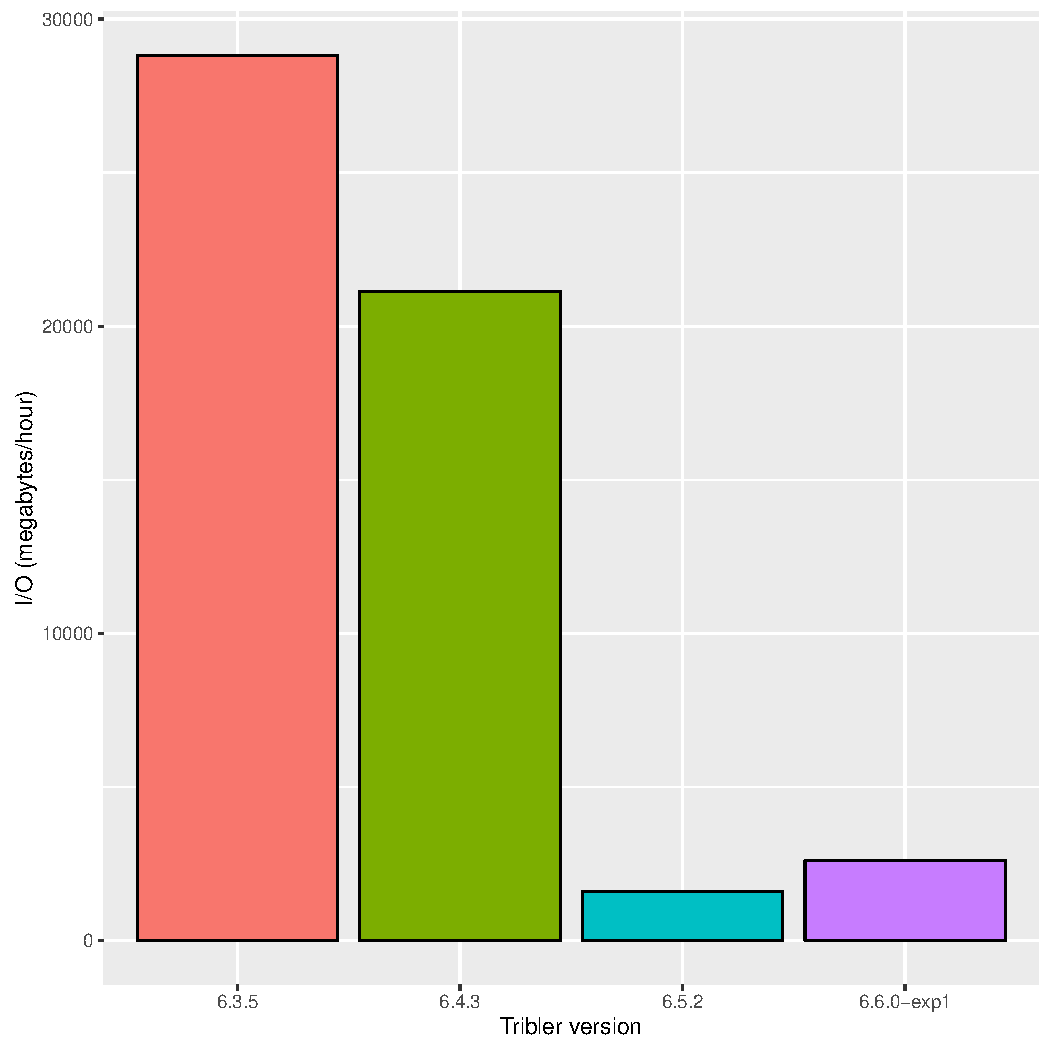
\includegraphics[width=\linewidth]{experimentation/images/io_history}
	\caption{The amount of I/O per version of Tribler.}
	\label{fig:io_history}
\end{figure} 

Each version of Tribler will run for one hour idle, using a clean state directory i.e. no prior knowledge of the network and its contents.
During the idle run, Tribler will start discovering peers and content such as channels and torrents, storing the obtained data in the database which gets flushed to disk.
Additionally, peers will start requesting data from this Tribler instance such as search and peer exchange requests, causing Tribler to read data from the database.
These read and writes operations will be monitored by iotop and the amounts automatically accumulated.
After one hour, the amount of read and write I/O is noted down and Tribler is shutdown.

The results of this experiment are visible in Figure~\ref{fig:io_history}.
From this figure we observe that Tribler's I/O has been reduced significantly in version 6.5.2.
This decrease was the result of batching multiple database queries and periodically flush them to disk, an effective optimization technique also applied in other work \cite{ouyang2011beyond, lin2009database}. 
Furthermore we observe the amount of I/O is increasing again in the latest 6.6.0-exp1 release due to the MultiChain feature added. 

Peculiarly, the numbers observed in this experiment are significantly higher than the numbers reported in the original ticket.
We believe the reason two reasons contribute to these numbers.
The first one is due to the 100 mbit connection of the experiment machine, providing excellent connectability conditions. 
Secondly, the fact that this instance began with a clean state directory while running idle, provides ideal conditions for Tribler to spend most of its resources on discovering peers and content.

\begin{table}[]
	\centering
	\caption{The packets collected for each version by Tribler when running idle for one hour using a clean state directory.}
	\label{table:packets_collected_idle}
	\begin{tabular}{|l|l|l|}
		\hline
		Paket type                         & Tribler version & Amount  \\ \hline
		\multirow{4}{*}{Dispersy-identity} & 6.3.5           & 20,026  \\ \cline{2-3} 
		& 6.4.3           & 38,268  \\ \cline{2-3} 
		& 6.5.2           & 46,890  \\ \cline{2-3} 
		& 6.6.0-exp1      & 41,480  \\ \hline
		\multirow{4}{*}{Dispersy-undo-own} & 6.3.5           & 40,594  \\ \cline{2-3} 
		& 6.4.3           & 45,095  \\ \cline{2-3} 
		& 6.5.2           & 47,409  \\ \cline{2-3} 
		& 6.6.0-exp1      & 44,279  \\ \hline
		\multirow{4}{*}{votecast}          & 6.3.5           & 44,990  \\ \cline{2-3} 
		& 6.4.3           & 90,339  \\ \cline{2-3} 
		& 6.5.2           & 116,557 \\ \cline{2-3} 
		& 6.6.0-exp1      & 96,509  \\ \hline
	\end{tabular}
\end{table}

To observe the cost versus the benefits, we have tracked the amount of packets Tribler managed to synchronize while running one hour idle using a clean state directory for each version.
The results are visible in Table~\ref{table:packets_collected_idle}.
From this table we conclude that while version 6.3.5 and 6.4.3 perform much more I/O, the amount of packets obtained is significantly less.
From these numbers we this conclude that the cost of having high I/O rates is not justified by the benefits as they perform even worse. 
Interestingly, the numbers of the latest 6.6.0-exp1 version are similar to that of 6.4.3, while we cannot explain this fully, we believe it may be caused by external network conditions or the MultiChain feature.

In conclusion, we believe that the I/O rate of Tribler does not show a correlation with the amount of packets synchronized. As the I/O rate of Tribler rises again in the latest version, possibly because of the MultiChain feature requiring additional computations, it shows the urgency of the I/O to become asynchronous and non-blocking.

\section{I/O breakdown}

\begin{table}[h]
	\centering
	\caption{Specifications of the setup used during the idle iotop measurement of Tribler 6.6.0-pre-exp.}
	\label{table:tribler_idle}
	\begin{tabular}{l|l}
		\hline
		\textbf{Packet type}	& \textbf{Amount} \\ \hline
		Operating System   	& Ubuntu 16.04 LTS \\
		Python version		& 2.7.12 \\
		CPU					& Intel Core i5-2410M \\ 
		HDD					& Samsung 850 EVO 250GB  \\ 
		RAM					& 8 GB DDR3 1600MHz \\
	\end{tabular}
\end{table}

\begin{table}[]
	\centering
	\caption{A breakdown of the Dispersy database function calls when running Tribler idle for one hour using a clean state directory.}
	\label{table:breakdown_tribler_idle}
	\begin{tabular}{|l|r|r|l|l|l|}
		\hline
		\textbf{Query}	& \textbf{Amount of calls} & \textbf{Total time (s)} & \textbf{Max}  & \textbf{Average} & \textbf{Min} \\ \hline
		execute			& 1,099,211	& 36.068 	& 0.24959	& 0.00003	& 0.00001 \\ \hline
		commit			& 65	& 11.089	& 1.12432	& 0.17061	& 0.00001 \\ \hline
		executemany		& 4282	& 0.233  	& 0.00071	& 0.00005	& 0.00001 \\ \hline
	\end{tabular}
\end{table}

To observe the individual components separately, we have created a breakdown of the database queries performed by Dispersy. \todo{Run this experiment on the ubuntu 15.10 machine.}

\section{Tribler's performance}

To measure the performance gain of Tribler, we have conducted two sets of experiments where two instances of Tribler, one with a synchronous, blocking Dispersy implementation and one with the asynchronous, non-blocking version of Dispersy, are compared.

In the first experiment we have ran Tribler idle for one hour while querying the Twisted event loop every 100 milliseconds for delayed calls.
By doing so we can observe if certain tasks have been delayed past their set time of execution i.e. measure the latency in the system.

In the second experiment we have stress-tested Tribler's new API.
By requesting data from an endpoint at several rates per second, we can observe the throughput, response times, variance in these response times and throughput of Tribler.

\subsection{Measuring the latency of Tribler}

\begin{figure}[!h]
	\centering
	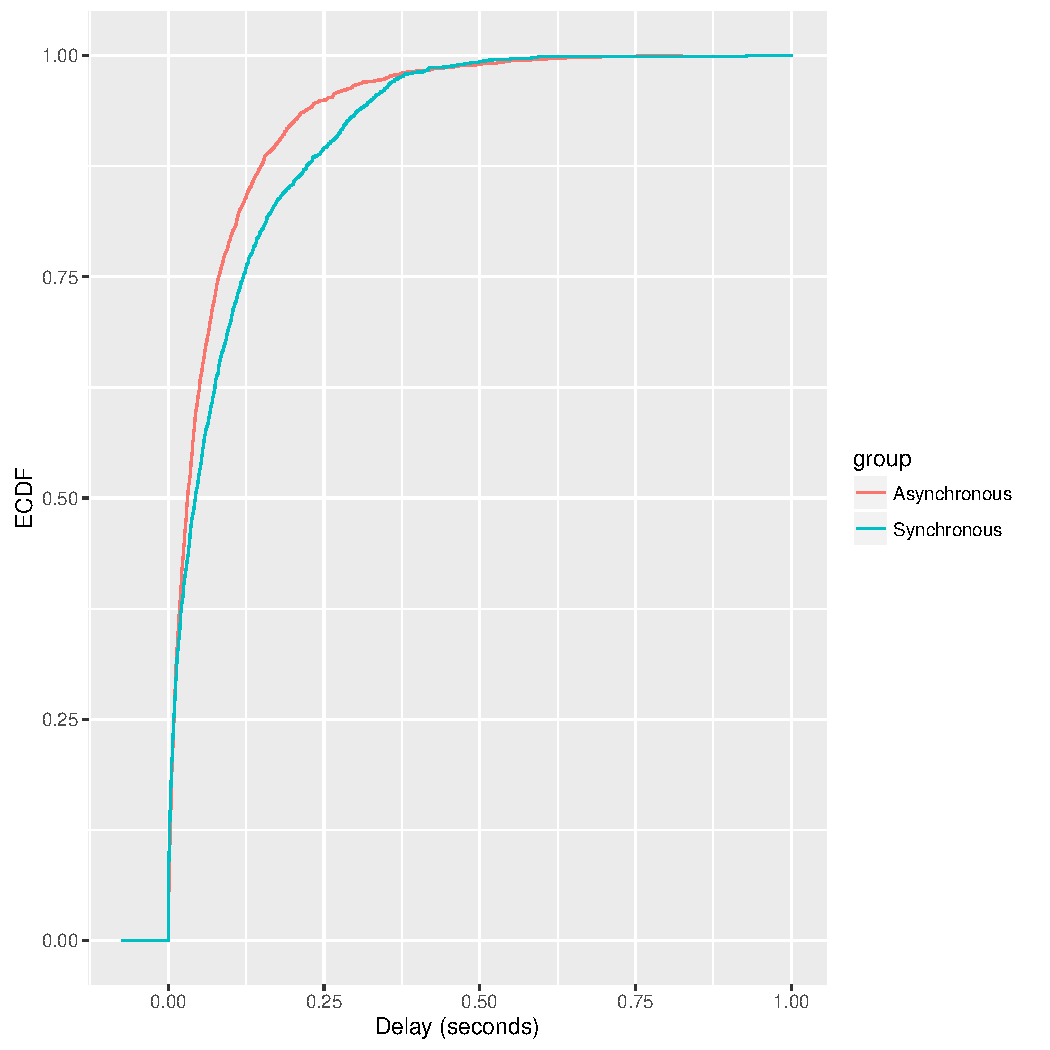
\includegraphics[width=\linewidth]{experimentation/images/ecdf_latency_idle}
	\caption{An ECDF plot of the latency when running Tribler idle.}
	\label{fig:ecdf_latency_idle}
\end{figure} 

In this experiment we have compared two versions of Tribler, one with Dispersy having blocking, synchronous I/O and one with Dispersy running StormDBManager and thus having non-blocking, asynchronous I/O.
Each instance of Tribler was run one hour idle where every 100 milliseconds the event loop of Twisted was queried for delayed calls.
By observing if scheduled calls are past their set time of execution, we can measure the amount of delay or \emph{latency} in the system.
Latency occurs when the twisted reactor thread is blocked or busy with a task that takes a relative long time to complete, causing other tasks to become delayed.
Latency is therefore directly related to the responsiveness of a program.
The lower the latency, the more responsive a system is.

In theory, making functions asynchronous slices them into smaller \enquote{chunks} which can be executed interleaved, creating a more responsive system as e.g. user actions will be executed in between (background) operations.

In this experiment the hypothesis is that the latency of the asynchronous version will be lower than its synchronous counterpart.
Since Tribler is running idle it has more resources i.e. CPU time available to tend to Dispersy which is running in the background, which most likely will cause the difference to be smaller than when Tribler is experiencing additional load.
However, we believe the average may still be significant enough to prefer the asynchronous implementation.

After running the experiment, we have created an empirical cumulative distribution function (ECDF) plot of the delayed calls, visible in Figure~\ref{fig:ecdf_latency_idle}.
From this figure we observe that the asynchronous version performs better than the synchronous version.
On average, the synchronous version has a latency of 87 milliseconds, where the asynchronous version has a latency of 66 milliseconds, a difference of 24\%.
Furthermore, the synchronous case has more outliers, some even touching the one second mark.
This observations are enough to confirm the hypothesis: both on average and in maxima the latency of the asynchronous version are lower.

\subsection{Measuring the responsiveness of Tribler}

To measure the responsiveness of Tribler while under load, we have stress tested the API of Tribler using the procedure described in Section~\ref{ssct:benchmark_3}.

In this experiment we use a state directory containing around 1200 channels.
By querying Tribler's channel API endpoint for all discovered channels, all channels in the database will be fetched and returned.
As this is Tribler's heaviest endpoint in terms of computation, it's the best way to put Tribler under load.
In total the experiment will be run six times, querying the channel endpoint exactly 1000 times per run using 1, 2, 5, 10, 15 and 20 requests per second respectively.
By tracking the response times, the amount of requests per seconds and the throughput the API can offer, we can measure the gain in responsiveness and thus in performance (T) of Tribler.
We expect that the asynchronous version will outperform the synchronous version significantly in both response times as throughput.

\begin{table}[!h]
	\centering
	\caption{The results of the six experiments runs with and without asynchronous, non-blocking I/O in Dispersy.}
	\label{table:responsiveness_tribler_load}
	\begin{tabular}{|c|c|c|c|c|c|c|c|}
		\hline
		Req./s              & Async. & Avg (ms) & Min & Max & Std. Dev. & T (KB/s) & Resp./s \\ \hline
		\multirow{2}{*}{1}  & \xmark      & 315 & 53  & 4774 & 615.90    & 564.19            & 0.9         \\ \cline{2-8} 
		& \cmark      & 134 & 57  & 2576 & 189.89    & 612.60            & 1.0         \\ \hline
		\multirow{2}{*}{2}  & \xmark       & 237 & 52  & 4524 & 475.31    & 1049.31           & 1.7         \\ \cline{2-8} 
		& \cmark      & 113 & 56  & 1224 & 162.62    & 1197.90           & 1.9         \\ \hline
		\multirow{2}{*}{5}  & \xmark       & 143 & 52  & 2865 & 259.64    & 2399.57           & 3.9         \\ \cline{2-8} 
		& \cmark      & 67  & 56  & 846  & 38.50     & 3058.27           & 5.0         \\ \hline
		\multirow{2}{*}{10} & \xmark       & 135 & 54  & 3338 & 259.37    & 3827.02           & 6.2         \\ \cline{2-8} 
		& \cmark      & 89  & 52  & 1138 & 92.58     & 5435.71           & 8.8         \\ \hline
		\multirow{2}{*}{15} & \xmark       & 133 & 51  & 4678 & 382.57    & 4521.46           & 7.3         \\ \cline{2-8} 
		& \cmark      & 88  & 52  & 963  & 82.23     & 6799.35           & 11.0        \\ \hline
		\multirow{2}{*}{20} & \xmark       & 109 & 51  & 3400 & 239.23    & 5599.75           & 9.1         \\ \cline{2-8} 
		& \cmark      & 74  & 52  & 1051 & 57.37     & 8264.01           & 13.4        \\ \hline
	\end{tabular}
\end{table}

\begin{figure}[!h]
	\centering
	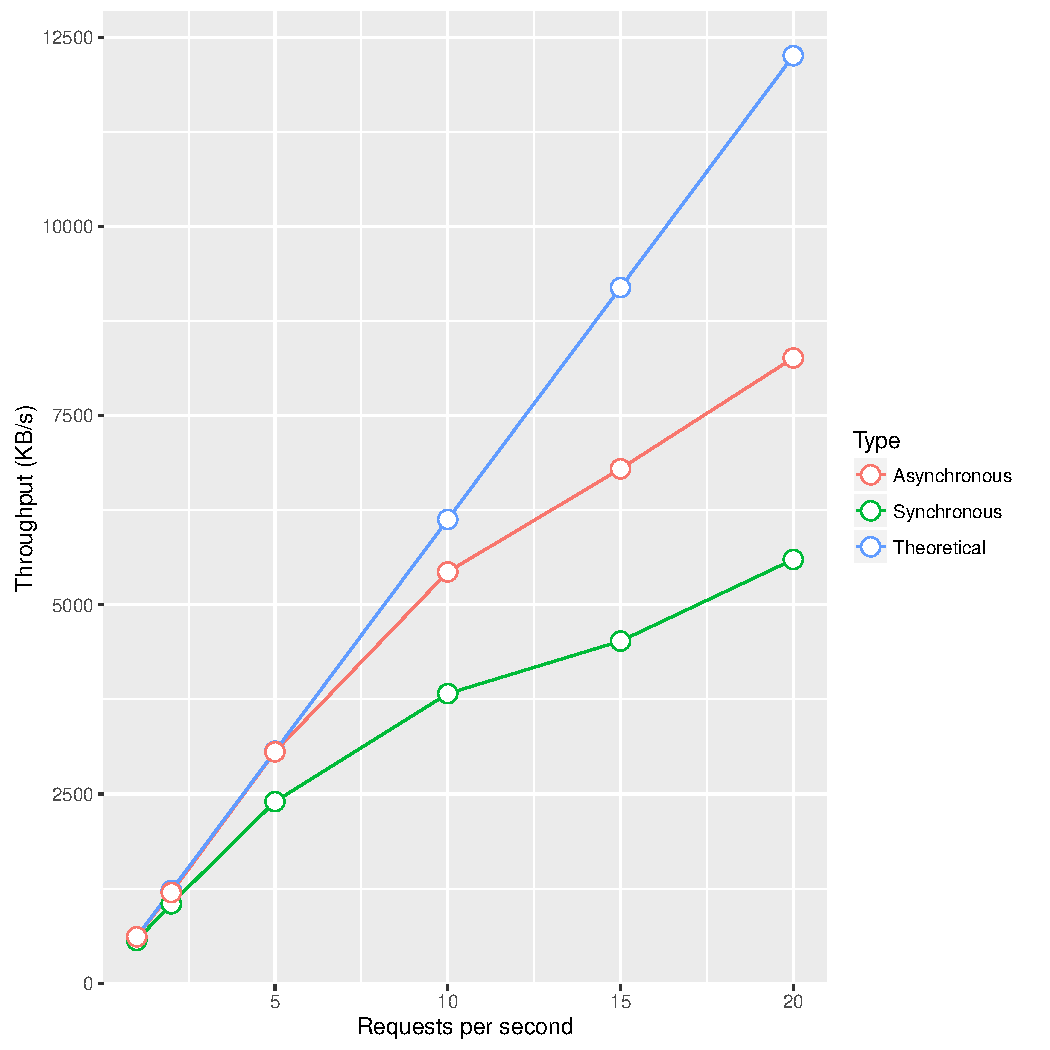
\includegraphics[width=\linewidth]{experimentation/images/throughput_requests.pdf}
	\caption{The throughput theoretically and of Tribler running Dispersy with asynchronous, non-blocking and synchronous, blocking I/O }
	\label{fig:throughput_requests}
\end{figure} 

The results of the experiment can be found in Table~\ref{table:responsiveness_tribler_load}.
From this table we observe that asynchronous version has a significant less amount of response time, both on average and in maximal duration.
The reduction in response times (on average) ranges between 32.1\% and 57.5\%.
As the responsiveness of a program can be directly linked to its performance (see Section~\ref{ssct:benchmark_3}), this looks very promising.
Interesting to note here is that the average response times of the synchronous version go down when the amount of requests per second goes up.
We believe this may be due to Twisted caching responses.

Another indication that the system has become more responsive is the the standard deviation.
For every run the standard deviation of the asynchronous version is significantly less than its synchronous counterpart, indicating the response times are more stable than the synchronous version. 
This can be explained by the slicing of tasks because of asynchrony; as tasks are more interleaved, smaller tasks such as a request will be processed in between bigger tasks, yielding a higher and more stable responsivity.

A third promising statistic is the throughput.
As the response is 613 kilobytes (KB) in size, the theoretical maximum throughput will be 613, 1226, 3065, 6130, 9195 and 12260 KB/s, respectively.
If we plot the theoretical, asynchronous and the synchronous throughput we obtain Figure~\ref{fig:throughput_requests}.
As we can see the throughput of the asynchronous case lies close to the theoretical maximum until around the ten requests per second.
At this point Tribler starts to show signs of being overloaded, which is also visible in the table when looking at the amount of responses received per second.

At ten requests per second both the asynchronous and the synchronous version cannot keep up.
If we look at the responses per second for fifteen and twenty requests per second, we observe that the gap between requests and responses grows percentage wise.
The question that arises here is why Tribler can't provide 13.4 responses per second with fifteen requests per second as in the case with twenty.
Again we believe the answer lies in the Twisted framework.

As more tasks are scheduled on the event loop of Twisted, it will process each of them fairly where priority is given to the most delayed task.
Since there are now more requests pending, it will spend more computation power on the requests.
Even though this means that more responses per second can be provided, percentage wise the amount of replies per request drops: for fifteen requests this percentage is 73\% where for twenty requests per second this percentage is 67\%.

All in all, this experiment demonstrates that the asynchronous system has superior performance over the synchronous case, increasing the throughput up to 150\%.

\subsection{Validating the performance regression test system}

\begin{figure}[!h]
	\centering
	\makebox[\textwidth][c]{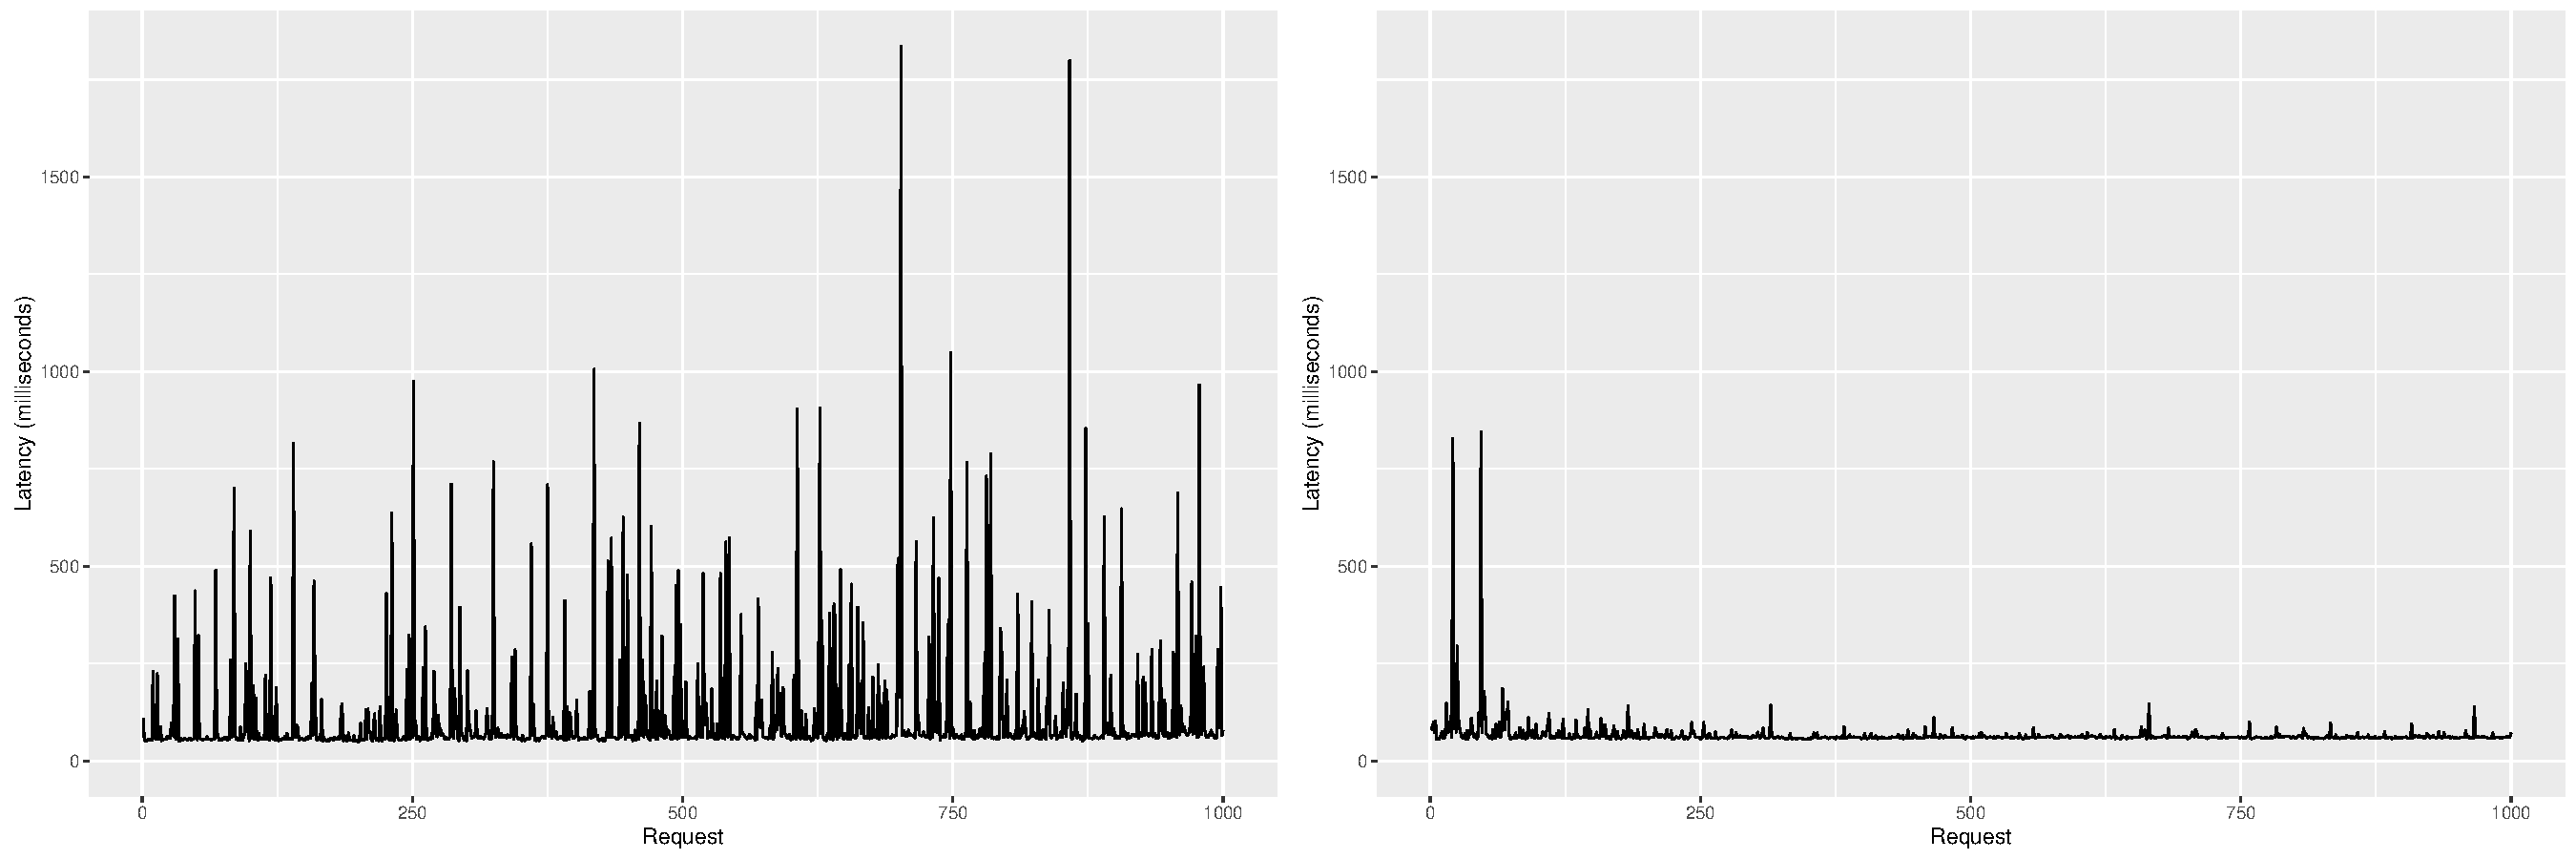
\includegraphics[width=0.9\paperwidth]{experimentation/images/response_times_comparison.pdf}}
	\caption{The comparison graph showing the response times of Tribler's API. Left: Tribler running Dispersy with synchronous, blocking I/O, right: Tribler running Dispersy with asynchronous, non-blocking I/O.}
	\label{fig:tribler_response_times_comparison}
\end{figure} 

To validate the performance regression system, we run the experiment above with 5 requests per second.
From the results, Gumby creates a side-by-side comparison graph and a table with an overview of the differences in the data obtained.

Figure~\ref{fig:tribler_response_times_comparison} shows the comparison graph generated.
From this figure, it is clear that the left hand side -- showing the current code base -- has higher response times than the right side.
From this graph it is immediately clear that the proposed changes have a positive impact on the responsiveness of the API.

To look at the data generated by the benchmark in more detail, the generated table shown in Figure~ \todo{todo} provides a breakdown of the data.
This breakdown highlights the average, minimum, maximum and standard deviation in response times as well as the throughput obtained.

From these figures we conclude that the performance regression test system provides a suitable overview for developers to get a quick overview of the current state.
%Conclusion
\chapter{Conclusion and Future Work}
\label{cpt:conclusion_and_future_work}

This thesis aims to contribute to the goal of re-decentralisation of systems such as Tribler to become as performant and as accessible as centralized solutions such as YouTube.
We have addressed Tribler's blocking database I/O, its main performance bottleneck, by integrating the Storm database framework into a new database manager: \enquote{StormDBManager}.
StormDBManager features a complete asynchronous, non-blocking interface for database access while still maintaining a serialized query execution strategy.
Furthermore we have provided deep insight into Tribler's and Dispersy's database usage, pinpointing functions that could be reviewed for query optimization.
By making Dispersy's database I/O asynchronous and non-blocking, we have improved Tribler's API throughput by up to 150\%, reduced its response times by up to 57.5\% and moved its longtail latencies to the 99th percentile up from the 90th percentile.

Additionally, we have created a regression testing system and prepared it to be integrated in our Jenkins continuous integration system to adopt software performance engineering in the development cycle, further maturing the project.
We have verified both the regression testing system and the resolving of the bottlenecks by providing experimental results.
We believe that with this performance boost and software performance engineering focus, we have contributed to Tribler's further years of research and strengthened Tribler's chances on becoming a decentralized alternative for YouTube-like streaming.

While we believe we made a significant step forward in both performance and software performance engineering, there are items left for future work.

As different platforms and operating systems may influence the performance of a program, it is useful to run regression tests on all platforms Tribler supports.
Deploying the regression test system on all platforms will ensure no regression occurs on one of them.

To remove the \enquote{raw queries} from all code bases, an object-relational mapping approach can be applied.
This will reduce the complexity of the system as all data will be contained in objects which are generally easier to modify and read from.
This will require extensive refactoring of Tribler and Dispersy's code bases.

While we have managed to move the longtail latencies to the 99th percentile and reduce the size of these latencies, there is still room for improvement.
Removing them completely by buffering or other means can lead to further improvements which could be investigated.

To improve performance further, moving Tribler from Python2 to Python3 is another possibility.
As we have seen, the Global Interpreter Lock in Python 3.2 and onwards has been updated to handle I/O-bound threads better.

To increase the speed of processing database queries, it can be investigated if we can use SQLite's multi-threaded support to process more queries.
While SQLite developers themselves admit SQLite has minimal multithreaded support, it can still be investigated to what extent we can leverage its support.

Improving the quality of Dispersy's tests is another item that was mentioned in this thesis.
It was found that passing all tests in Dispersy does not provide any guarantees beyond a basic level of correctness.
Improving and adding tests is required to increase the stability, maintainability and correctness of Dispersy.

A final item that we would like to highlight as future work is running benchmarks in a closed environment, disconnected from the Internet.
When running Tribler and Dispersy, it will connect to the Internet which may influence performance metrics such as I/O rates and amount of packets obtained.
Creating a closed environment with local peers will ensure that only those peers can communicate to one another.
These peers can then be instrumented to behave in a predetermined manner.
This will increase both the reliability and accuracy of the measurements made.



% BIBLIOGRAPHY
%\bibliographystyle{bib/latex8}
\bibliography{bib/bibliography}

\appendix

\appendix


\end{document}

